\batchmode
\makeatletter
\def\input@path{{/home/rgiordan/Documents/git_repos/CovariancesRobustnessVBPaper/writing/}}
\makeatother
\documentclass{article}\usepackage[]{graphicx}\usepackage[]{color}
%% maxwidth is the original width if it is less than linewidth
%% otherwise use linewidth (to make sure the graphics do not exceed the margin)
\makeatletter
\def\maxwidth{ %
  \ifdim\Gin@nat@width>\linewidth
    \linewidth
  \else
    \Gin@nat@width
  \fi
}
\makeatother

\definecolor{fgcolor}{rgb}{0.345, 0.345, 0.345}
\newcommand{\hlnum}[1]{\textcolor[rgb]{0.686,0.059,0.569}{#1}}%
\newcommand{\hlstr}[1]{\textcolor[rgb]{0.192,0.494,0.8}{#1}}%
\newcommand{\hlcom}[1]{\textcolor[rgb]{0.678,0.584,0.686}{\textit{#1}}}%
\newcommand{\hlopt}[1]{\textcolor[rgb]{0,0,0}{#1}}%
\newcommand{\hlstd}[1]{\textcolor[rgb]{0.345,0.345,0.345}{#1}}%
\newcommand{\hlkwa}[1]{\textcolor[rgb]{0.161,0.373,0.58}{\textbf{#1}}}%
\newcommand{\hlkwb}[1]{\textcolor[rgb]{0.69,0.353,0.396}{#1}}%
\newcommand{\hlkwc}[1]{\textcolor[rgb]{0.333,0.667,0.333}{#1}}%
\newcommand{\hlkwd}[1]{\textcolor[rgb]{0.737,0.353,0.396}{\textbf{#1}}}%
\let\hlipl\hlkwb

\usepackage{framed}
\makeatletter
\newenvironment{kframe}{%
 \def\at@end@of@kframe{}%
 \ifinner\ifhmode%
  \def\at@end@of@kframe{\end{minipage}}%
  \begin{minipage}{\columnwidth}%
 \fi\fi%
 \def\FrameCommand##1{\hskip\@totalleftmargin \hskip-\fboxsep
 \colorbox{shadecolor}{##1}\hskip-\fboxsep
     % There is no \\@totalrightmargin, so:
     \hskip-\linewidth \hskip-\@totalleftmargin \hskip\columnwidth}%
 \MakeFramed {\advance\hsize-\width
   \@totalleftmargin\z@ \linewidth\hsize
   \@setminipage}}%
 {\par\unskip\endMakeFramed%
 \at@end@of@kframe}
\makeatother

\definecolor{shadecolor}{rgb}{.97, .97, .97}
\definecolor{messagecolor}{rgb}{0, 0, 0}
\definecolor{warningcolor}{rgb}{1, 0, 1}
\definecolor{errorcolor}{rgb}{1, 0, 0}
\newenvironment{knitrout}{}{} % an empty environment to be redefined in TeX

\usepackage{alltt}
\usepackage[latin9]{inputenc}
\usepackage{geometry}
\geometry{verbose}
\usepackage{verbatim}
\usepackage{prettyref}
\usepackage{url}
\usepackage{amsmath}
\usepackage{amsthm}
\usepackage{amssymb}
\usepackage{graphicx}
\usepackage[authoryear]{natbib}
\usepackage{xargs}[2008/03/08]
\usepackage[unicode=true,
 bookmarks=false,
 breaklinks=false,pdfborder={0 0 1},backref=section,colorlinks=false]
 {hyperref}

\makeatletter

%%%%%%%%%%%%%%%%%%%%%%%%%%%%%% LyX specific LaTeX commands.
%% Because html converters don't know tabularnewline
\providecommand{\tabularnewline}{\\}

%%%%%%%%%%%%%%%%%%%%%%%%%%%%%% Textclass specific LaTeX commands.
\theoremstyle{plain}
\newtheorem{thm}{\protect\theoremname}[section]
  \theoremstyle{definition}
  \newtheorem{defn}[thm]{\protect\definitionname}
  \theoremstyle{plain}
  \newtheorem{cor}[thm]{\protect\corollaryname}
  \theoremstyle{plain}
  \newtheorem{assumption}[thm]{\protect\assumptionname}
  \theoremstyle{plain}
  \newtheorem{prop}[thm]{\protect\propositionname}
  \theoremstyle{plain}
  \newtheorem{lem}[thm]{\protect\lemmaname}

%%%%%%%%%%%%%%%%%%%%%%%%%%%%%% User specified LaTeX commands.
% For LaTeX2e

% Set to togglefalse to use nips formatting.
% Set to toggletrue to use arxiv formatting.
%\usepackage{etoolbox}
%\newtoggle{arxivformat}

\usepackage{times}

\usepackage{url}

\usepackage{subcaption}
\usepackage{caption}

\usepackage{amsthm}
\usepackage{appendix}

% break equations across pages
%\allowdisplaybreaks

% Used to number single equations in an equation array.
\newcommand{\numberthis}{\addtocounter{equation}{1}\tag{\theequation}}

\usepackage{bbm}


% references
% Since many figures and labels are generated by Knitr, we cannot always use
% Lyx's cross references. 
\newcommand{\fig}[1]{Fig.~(\ref{fig:#1})}

% Custom references for prettyref
\newrefformat{app}{Appendix \ref{#1}}
\newrefformat{eq}{Eq.~(\ref{#1})}
\newrefformat{assu}{Assumption~(\ref{#1})}
\newrefformat{subsec}{Section~(\ref{#1})}
\newrefformat{cor}{Corollary~(\ref{#1})}
\newrefformat{thm}{Theorem~(\ref{#1})}
\newrefformat{def}{Definition~(\ref{#1})}
\newrefformat{prop}{Proposition~(\ref{#1})}
\newrefformat{tab}{Table~(\ref{#1})}

% theorems
%\theoremstyle{plain}
%\newtheorem{theorem}{}[section]
%\newtheorem{proposition}[theorem]{}\newtheorem{lemma}[theorem]{}\newtheorem{remark}[theorem]{}

\title{Covariances, Robustness, and Variational Bayes}

\author{
Ryan Giordano\\
Department of Statistics\\
UC Berkeley
%University of California, Berkeley
%Berkeley, CA 94720 \\
%\texttt{rgiordano@berkeley.edu}
\and
Tamara Broderick \\
Department of EECS\\
MIT
%Cambridge, MA 02139\\
%\texttt{tbroderick@csail.mit.edu}
\and
Michael I. Jordan \\
Departments of EECS and Statistics\\
UC Berkeley
%University of California, Berkeley\\
%Berkeley, CA 94720 \\
%\texttt{jordan@cs.berkeley.edu }
}

\newcommand{\fix}{\marginpar{FIX}}
\newcommand{\new}{\marginpar{NEW}}

\makeatother

  \providecommand{\assumptionname}{Assumption}
  \providecommand{\corollaryname}{Corollary}
  \providecommand{\definitionname}{Definition}
  \providecommand{\lemmaname}{Lemma}
  \providecommand{\propositionname}{Proposition}
\providecommand{\theoremname}{Theorem}
\IfFileExists{upquote.sty}{\usepackage{upquote}}{}
\begin{document}
\maketitle

\begin{comment}
Math macros
\end{comment}

\begin{comment}
Basics
\end{comment}

\global\long\def\constant{Constant}

\newcommandx\tconst[1][usedefault, addprefix=\global, 1=t]{C_{#1}}

\global\long\def\trans{\intercal}

\global\long\def\mbe{\mathbb{E}}

\global\long\def\indep{\stackrel{indep}{\sim}}

\global\long\def\iid{\stackrel{iid}{\sim}}

\global\long\def\kl{\mathrm{KL}}

\global\long\def\cov{\mathrm{Cov}}

\global\long\def\var{\mathrm{Var}}

\global\long\def\normal{\mathcal{N}}

\global\long\def\argmin{\operatornamewithlimits{argmin}}

\global\long\def\argmax{\operatornamewithlimits{argmax}}

\begin{comment}
Distributions
\end{comment}

\newcommandx\pthetapost[1][usedefault, addprefix=\global, 1=\alpha]{p_{#1}^{x}}

\newcommandx\qthetapost[1][usedefault, addprefix=\global, 1=\alpha]{q_{#1}^{x}}

\newcommandx\prior[2][usedefault, addprefix=\global, 1=\theta, 2=\alpha]{p\left(#1\vert#2\right)}

\global\long\def\ptthetapost{\pthetapost[\alpha,t]}

\global\long\def\qtthetapost{\qthetapost[\alpha,t]}

\global\long\def\etaopt{\eta^{*}}

\global\long\def\etatopt{\eta^{*}\left(t\right)}

\global\long\def\qthetapostarg{\qthetapost\left(\theta;\eta^{*}\right)}

\global\long\def\qtthetapostarg{\qthetapost\left(\theta;\eta^{*}\left(t\right)\right)}

\newcommandx\gtheta[1][usedefault, addprefix=\global, 1=\theta]{g\left(#1\right)}

\global\long\def\mbeq{\mbe_{\qthetapost}}

\global\long\def\mbep{\mbe_{\pthetapost}}

\global\long\def\epgtheta{\mbe_{\pthetapost}\left[\gtheta\right]}

\global\long\def\eqgtheta{\mbe_{\qthetapost}\left[\gtheta\right]}

\global\long\def\lrvbcov{\mathrm{Cov}_{\qthetapost}^{LR}}

\global\long\def\klhess{\mathbf{H}_{\eta\eta}}

\global\long\def\efhess{\mathbf{f}_{t\eta}}

\global\long\def\eggrad{\mathbf{g}_{\eta}}

\global\long\def\covmat{\boldsymbol{\Sigma}}

\global\long\def\infomat{\boldsymbol{\Lambda}}

\begin{comment}
Sensitivity
\end{comment}

\global\long\def\psens{\mathbf{S}_{\alpha}}

\global\long\def\qsens{\mathbf{S}_{\alpha}^{q}}

\global\long\def\psenshat{\hat{\mathbf{S}}_{\alpha}}

\global\long\def\contampriornoarg{u}

\newcommandx\contamprior[1][usedefault, addprefix=\global, 1=\theta]{\contampriornoarg\left(#1\right)}

\global\long\def\psensfunc{S_{\contampriornoarg}}

\global\long\def\qsensfunc{S_{\contampriornoarg}^{q}}

\global\long\def\qsenssup{S_{sup}^{q}}

\global\long\def\psenssup{S_{sup}}

\global\long\def\contamnorm{C_{u}}

\newcommandx\origprior[1][usedefault, addprefix=\global, 1=\theta]{p_{0}\left(#1\right)}

\newcommandx\influence[2][usedefault, addprefix=\global, 1=\phantom{}, 2=\phantom{}]{I_{#2}^{#1}\left(\theta\right)}

\global\long\def\influenceplus{\influence[+]}

\newcommandx\qinfluence[1][usedefault, addprefix=\global, 1=\phantom{}]{\influence[#1][q]}

\newcommandx\covdens[2][usedefault, addprefix=\global, 1=\theta, 2=t]{\rho\left(#1,#2\right)}

\newcommandx\covdensnorm[2][usedefault, addprefix=\global, 1=\theta, 2=t]{p\left(#1\vert#2\right)}

\newcommandx\linearoperator[2][usedefault, addprefix=\global, 1=\theta, 2={\,}]{L^{#2}\left(#1\right)}

\begin{comment}
Laplace and EM
\end{comment}

\global\long\def\laptheta{\hat{\theta}_{Lap}}

\global\long\def\laphess{\mathbf{H}_{Lap}}

\global\long\def\lap{p_{Lap,\alpha}^{x}}

\global\long\def\lapgtheta{g_{\laptheta}}


\begin{abstract}
Variational Bayes (VB) is an approximate Bayesian posterior inference
technique that is increasingly popular due to its fast runtimes on
large-scale datasets. However, even when VB provides accurate posterior
means for certain parameters, it often mis-estimates variances and
covariances. Furthermore, prior robustness measures have remained
undeveloped for VB. By deriving a simple formula for the effect of
infinitesimal model perturbations on VB posterior means, we provide
both improved covariance estimates and local robustness measures for
VB, thus greatly expanding the practical usefulness of VB posterior
approximations. The estimates for VB posterior covariances rely on
a result from the classical Bayesian robustness literature relating
derivatives of posterior expectations to posterior covariances. Our
key assumption is that the VB approximation provides good estimates
of a select subset of posterior means\textemdash an assumption that
has been shown to hold in many practical settings. In our experiments,
we demonstrate that our methods are simple, general, and fast, providing
accurate posterior uncertainty estimates and robustness measures with
runtimes that can be an order of magnitude  smaller than MCMC.

Key phrases: Variational Bayes; Bayesian robustness; Mean field approximation;
Linear response theory; Automatic differentiation
\end{abstract}

\section{Introduction\label{sec:intro} }

Most Bayesian posteriors cannot be calculated analytically, so in
practice we turn to approximations. Variational Bayes (VB) casts posterior
approximation as an optimization problem in which the objective to
be minimized is the divergence, among a tractable sub-class of posteriors,
from the exact posterior. For example, one widely-used and relatively
simple flavor of VB is ``mean field variational Bayes'' (MFVB),
which employs Kullback-Liebler (KL) divergence and a factorizing exponential
family approximation for the tractable sub-class of posteriors \citep{wainwright2008graphical}.
MFVB has been increasingly popular as an alternative to Markov Chain
Monte Carlo (MCMC) in part due to its fast runtimes on large-scale
data sets. Although MFVB does not come with any general accuracy guarantees
(except asymptotic ones in special cases, as in \citet{westling:2015:vbconsistency,wang:2017:vbconsistency}),
MFVB produces posterior mean estimates of certain parameters that
are accurate enough to be useful in a number of real-world applications
\citep{blei:2016:variational}. In the current work we will focus
on MFVB for motivation and in our examples and experiments, though
many of the ideas here could be applied to more general approximations
or divergences. Despite its computational advantages, MFVB typically
underestimates marginal variances \citep{mackay:2003:information,wang:2005:inadequacy,turner:2011:two},
and, to our knowledge, techniques for assessing Bayesian robustness
have not yet been developed for VB.  It is these inferential issues
that arethe focus of the current paper.

In contrast to the optimization approach of VB, MCMC constructs a
Markov chain with the exact posterior as its stationary distribution.
At first glance, it may seem that MCMC is made for integration and
MFVB is made for differentiation. Using MCMC draws, integrals with
respect to the posterior can be readily approximated by constructing
the corresponding sample moment from the MCMC draws. Similarly, as
a parametric optimization problem, MFVB lends itself naturally to
sensitivity analysis, since its optimum can be differentiated analytically.
However, a key result of the Bayesian local robustness literature
is that derivatives and covariances are two sides of the same coin,
since, under mild regularity conditions, derivatives of posterior
quantities can re-cast as posterior covariances by exchanging the
order of integration and differentiation (\citet{gustafson:1996:localposterior,basu:1996:local,efron:2015:frequentist}
and \prettyref{subsec:cov_and_sens} below). 

Thus, in order to calculate local prior sensitivity, the Bayesian
robustness literature re-casts prior sensitivities as posterior covariances
that can be easily calculated with MCMC. In order to provide covariance
estimates for MFVB, we turn this idea on its head and use the sensitivity
of MFVB posterior expectations to estimate their covariances. Additionally,
we derive straightforward general VB (not only MFVB) versions of a
number of prior sensitivity measures from the Bayesian robustness
literature, including parametric sensitivity and sensitivity to additive
functional perturbations. Our key assumption is that the posterior
means of interest are well-estimated by VB for all the perturbations
of interest. In our experiments, we compare MFVB models to both MCMC
and maximum a posteriori (MAP) posterior approximations. We find that
the MFVB means and variances, unlike the MAP estimates, match the
MCMC approximations closely while still running over an order of magnitude
faster than MCMC.

We will begin in \prettyref{sec:theory} by discussing the general
relationship between Bayesian sensitivity and posterior covariance,
and then defining local robustness and sensitivity. Next, we will
introduce VB and derive the linear system for the VB local sensitivity
estimates. In \prettyref{sec:sensitivity_in_action}, we show how
to use the VB local sensitivity results to estimate covariances and
calculate a range of canonical Bayesian prior sensitivity measures.
Finally, in \prettyref{sec:experiments}, we describe our experiments
on real industry data that illustrate the speed and effectiveness
of our methods. \prettyref{sec:Conclusion} concludes.

\section{Bayesian (and variational Bayesian) covariances and sensitivity\label{sec:theory}}

An MCMC posterior estimate is an empirical distribution formed with
posterior draws, and a VB posterior estimate takes the form of a parameterized
distribution with optimized parameters. MCMC draws lend themselves
naturally to the approximate calculation of posterior moments, such
as those required for covariances. In contrast, VB approximations
lend themselves naturally to sensitivity analysis, since we can analytically
differentiate the optima with respect to perturbations. However, the
contrast between derivatives and moments is not so stark since, under
mild regularity conditions that allow the exchange of integration
and differentiation, there is a direct correspondence between sensitivity
and covariance. Thus, as has long been known in the Bayesian robustness
literature, we can use the sample covariances of MCMC to calculate
posterior sensitivities. With VB approximations, for which sensitivity
is more natural, we can apply this relationship in reverse: we can
use the VB sensitivity to calculate covariances.

\subsection{Covariances and sensitivity\label{subsec:cov_and_sens}}

We will first state a general result relating sensitivity and covariance
and apply it to our specific cases of interest as they arise throughout
the paper. Denote an unknown model parameter by the vector $\theta\in\mathbb{R}^{K}$,
and assume a dominating measure for $\theta$ given by $\lambda$.
Define $\covdens$ to be any $\lambda$-measurable function on $\theta$
that depends on an index $t\in\mathbb{R}^{D}$, and assume that $0<\int\exp\left(\rho\left(\theta,t\right)\right)\lambda\left(d\theta\right)<\infty$.
For our purposes, one may think of $\exp\left(\covdens\right)$ as
the product of a parameterized likelihood and a prior with dependencies
other than $t$ left implicit. Later on, we will choose $t$ and $\rho\left(\theta,t\right)$
to represent various prior and model perturbations, but for now we
will keep the discussion abstract. After normalization we get a density,
$\covdensnorm$, in $\theta$ with respect to $\lambda$ : 
\begin{align*}
\covdensnorm & :=\frac{\exp\left(\covdens\right)}{\int\exp\left(\covdens[\theta']\right)\lambda\left(d\theta'\right)}.
\end{align*}
 Suppose we are interested in differentiating the expectation
\begin{align*}
\mbe_{\covdensnorm}\left[g\left(\theta\right)\right] & :=\int\covdensnorm\gtheta\lambda\left(d\theta\right)
\end{align*}
with respect to $t$ at $t=0$. This will measure the local sensitivity
of $\mbe_{\covdensnorm}\left[g\left(\theta\right)\right]$ to the
index $t$ at $t=0$.
\begin{thm}
\label{thm:sens_cov}

When \prettyref{assu:exchange_order} and \prettyref{assu:bayes_ok}
hold for all $t$ in a neighborhood of zero, then
\begin{align}
\left.\frac{d\mbe_{\covdensnorm}\left[g\left(\theta\right)\right]}{dt^{\trans}}\right|_{t=0} & =\cov_{\covdensnorm[][0]}\left(g\left(\theta\right),\left.\frac{\partial\covdens}{\partial t}\right|_{t=0}\right).\label{eq:covariance_sensitivity_general}
\end{align}
\end{thm}

See \prettyref{app:sens_and_cov} for a proof and technical conditions.
By using MCMC draws to calculate the covariance on the right-hand
side of \prettyref{eq:covariance_sensitivity_general}, one can form
an estimate of $d\mbe_{\covdensnorm}\left[g\left(\theta\right)\right]/dt^{\trans}$
at $t=0$. One might also approach the problem of calculating $d\mbe_{\covdensnorm}\left[g\left(\theta\right)\right]/dt^{\trans}$
using importance sampling \citep[Chapter 9]{owen:2013:mcmcbook} as
follows. First, an importance sampling estimate of the dependence
of $\mbe_{\covdensnorm}\left[\gtheta\right]$ on $t$ can be constructed
with weights that depend on $t$. Then, by differentiating the weights
with respect to $t$, this would provide a sample-based estimate of
$d\mbe_{\covdensnorm}\left[g\left(\theta\right)\right]/dt^{\trans}$.
We show in \prettyref{app:mcmc_importance_sampling} that this is
approach is equivalent to using MCMC samples to estimate the covariance
in \prettyref{thm:sens_cov}.

In \prettyref{subsec:local_sensitivity}, \prettyref{thm:sens_cov}
will immediately allow us to calculate local sensitivity from MCMC
draws using sample covariances. After a little more work, in \prettyref{subsec:lrvb_cov},
\prettyref{thm:sens_cov} will allow us to use the sensitivity of
VB means to calculate their covariances.

\subsection{Local sensitivity and robustness\label{subsec:local_sensitivity}}

As in \prettyref{subsec:cov_and_sens}, denote an unknown model parameter
by the vector $\theta\in\mathbb{R}^{K}$, and assume a dominating
measure on $\theta$ given by $\lambda$. Denote the prior parameters
by $\alpha$, where $\alpha\in\mathbb{R}^{M}$. Finally, denote our
data by $x$. Suppose we have tentatively chosen a likelihood, $p\left(x\vert\theta\right)$,
and a prior, $\prior$. We then let $\pthetapost$ denote the posterior
distribution of $\theta$ given $x$, as given by Bayes' Theorem:
\begin{align*}
\pthetapost\left(\theta\right) & :=p\left(\theta\vert x,\alpha\right)=\frac{p\left(x\vert\theta\right)\prior}{\int p\left(x\vert\theta'\right)\prior[\theta']\lambda\left(d\theta'\right)}.
\end{align*}
We will assume that we are interested in a posterior expectation of
some function $\gtheta$ (e.g., a parameter mean, a posterior predictive
value, or squared loss): $\epgtheta$. In the current work, we will
quantify the uncertainty of $\epgtheta$ by the posterior variance,
$\var_{\pthetapost}\left(\gtheta\right)$. Other measures of central
tendency (e.g., posterior medians) or uncertainty (e.g., posterior
quantiles) may also be good choices, but are beyond the scope of the
current work.

Note the dependence of $\epgtheta$ on both the likelihood and prior
through Bayes' theorem. The choice of a prior and choice of a likelihood
is made by the modeler and is almost invariably a simplified representation
of the real world. The choice is therefore to some extent subjective,
and so one hopes that the salient aspects of the posterior would not
vary under reasonable variation in the choice of prior and the choice
of likelihood. Consider the prior, for example: the process of prior
elicitation may be prohibitively time-consuming; two practitioners
may have irreconcilable subjective prior beliefs; or the model may
be so complex and high-dimensional that humans cannot reasonably express
their prior beliefs as formal distributions. All of these circumstances
might give rise to a range of reasonable prior choices. A posterior
quantity is ``robust'' to the prior to the extent that it does not
change much when calculated under these different prior choices. Although
robustness to the likelihood is no less important, in this paper we
will focus on prior robustness, in part for continuity with existing
literature.

Quantifying the sensitivity of the posterior to variation in the likelihood
and prior is one of the central concerns of the field of robust Bayes
\citep{berger:2012:robust}. (We will not discuss the other central
concern, which is the selection of priors and likelihoods that lead
to robust estimators.) Suppose that we have determined that the prior
parameter $\alpha$ belongs to some set $\mathcal{A}$, perhaps after
expert prior elicitation. Ideally, we would calculate the extrema
of $\epgtheta$ as $\alpha$ ranges over all of $\mathcal{A}$. This
is called \textit{global robustness} and is intractable or difficult
except in special cases \citep[Chapter 15]{moreno:2012:globalrobustness,huber:2011:robust}.
An alternative is to examine how much $\epgtheta$ changes locally
in response to small perturbations in the value of $\alpha$. To this
end, we define the \textit{local sensitivity} \citep{gustafson:2012:localrobustnessbook}:
\begin{defn}
The local sensitivity of $\epgtheta$ to prior parameter $\alpha$
is given by

\begin{eqnarray}
\psens & := & \left.\frac{d\epgtheta}{d\alpha}\right|_{\alpha}.\label{eq:local_robustness}
\end{eqnarray}
$\psens$, the local sensitivity, can be considered a measure of\emph{
local robustness} \citep{gustafson:2012:localrobustnessbook}. Throughout
the paper we will distinguish between sensitivity, which comprises
objectively defined quantities such as $\psens$, and robustness,
which we treat as a more subjective decision that may be informed
by the sensitivity as well as other considerations. For example, even
if one knows $\psens$ precisely, how much posterior change is too
much change and how much prior variation is reasonable remain decisions
to be made by the modeler. For a more in-depth discussion of how we
use the terms sensitivity and robustness, see \prettyref{app:sens_and_robustness}.

 Local sensitivity can be thought of as quantifying sensitivity to
priors within a small region where the posterior dependence on the
prior is approximately linear. It provides an approximation to global
robustness in the sense that, to first order, for $\Delta\alpha\in\mathcal{A}-\alpha$,
\begin{align*}
\left.\epgtheta\right|_{\alpha+\Delta\alpha} & \approx\epgtheta+\psens^{\trans}\Delta\alpha.
\end{align*}
\end{defn}

An immediate corollary of \prettyref{thm:sens_cov} allows us to calculate
$\psens$ as a  covariance.
\begin{cor}
\label{cor:sens_cov_prior}

When the conditions of \prettyref{thm:sens_cov} hold for $t=\alpha$
and $\covdens[][\alpha]=\log p\left(x\vert\theta\right)+\log\prior$
then
\begin{align}
\psens & =\cov_{\pthetapost}\left(\gtheta,\frac{\partial\log\prior}{\partial\alpha}\right).\label{eq:covariance_sensitivity}
\end{align}
\end{cor}

See also \citet{basu:1996:local}, in which \prettyref{cor:sens_cov_prior}
is stated in the proof of Theorem 1, as well as \citet{perez:2006:mcmc}
and \citet{efron:2015:frequentist}. Given MCMC draws from a chain
we assume to have reached equilibrium with stationary distribution
$\pthetapost$, one can calculate an estimate of $\psens$ using the
sample covariance version of \prettyref{eq:covariance_sensitivity_general}:
\begin{align}
\psenshat & :=\frac{1}{N_{s}}\sum_{n=1}^{N_{s}}g\left(\theta_{n}\right)\frac{\partial\log\prior[\theta_{n}]}{\partial\alpha^{\trans}}-\left(\frac{1}{N_{s}}\sum_{n=1}^{N_{s}}g\left(\theta_{n}\right)\right)\left(\frac{1}{N_{s}}\sum_{n=1}^{N_{s}}\frac{\partial\log\prior[\theta_{n}]}{\partial\alpha^{\trans}}\right)\label{eq:mcmc_sample_cov}\\
\textrm{for }\theta_{n} & \iid\pthetapost\left(\theta\right),\textrm{ for }n=1,...,N_{s}.\nonumber 
\end{align}

\subsection{Variational Bayes\label{subsec:variational_Bayes}}

We now briefly review VB and state our key assumptions about its accuracy.
We wish to find an approximate distribution, in some class $\mathcal{Q}$
of tractable distributions, selected to minimize the Kullback-Liebler
divergence (KL divergence) between $q\in\mathcal{Q}$ and the exact
posterior $\pthetapost$. We assume that distributions in $\mathcal{Q}$
are parameterized by a finite-dimensional parameter $\eta$ in some
feasible set $\Omega_{\eta}\subseteq\mathbb{R}^{K_{\eta}}$:
\begin{eqnarray}
\mathcal{Q} & := & \left\{ q:q=q\left(\theta;\eta\right)\textrm{ for }\eta\in\Omega_{\eta}\right\} .\label{eq:q_approximating_family}
\end{eqnarray}
Given $\mathcal{Q}$, we define the optimal $q\in\mathcal{Q}$, which
we call $\qthetapost$, as that distribution that minimizes the KL
divergence $KL\left(q\left(\theta;\eta\right)||\pthetapost\left(\theta\right)\right)$
from $\pthetapost$. We denote the corresponding optimal variational
parameters as $\etaopt$.
\begin{defn}
The variational approximation $\qthetapost\left(\theta\right)$ to
$\pthetapost\left(\theta\right)$ is defined by

\begin{eqnarray}
\qthetapost\left(\theta\right)=q\left(\theta;\etaopt\right) & := & \textrm{argmin}_{q\in\mathcal{Q}}\left\{ KL\left(q\left(\theta;\eta\right)||\pthetapost\left(\theta\right)\right)\right\} \label{eq:kl_divergence}
\end{eqnarray}
where
\begin{align*}
KL\left(q\left(\theta;\eta\right)||\pthetapost\left(\theta\right)\right) & =\mbe_{q\left(\theta;\eta\right)}\left[\log q\left(\theta;\eta\right)-\log p\left(x\vert\theta\right)-\log p\left(\theta\vert\alpha\right)\right]+\log p\left(x\right).
\end{align*}
\end{defn}

In the KL divergence, the (generally intractable) normalizing term
$\log p\left(x\right)$ does not depend on $q\left(\theta\right)$
and so can be neglected in the optimization. In order for the KL divergence
to be well defined, we assume that both $p\left(\theta\right)$ and
$q\left(\theta\right)$ are given with respect to the same base measure,
$\lambda$, and that the support of $q\left(\theta\right)$ is contained
in the support of $p\left(\theta\right)$. We additionally assume
that $KL\left(q\left(\theta;\eta\right)||\pthetapost\left(\theta\right)\right)$
is twice differentiable as a function of $\eta$, that the optimal
$\etaopt$ is interior to $\Omega_{\eta}$, and that $\etaopt$ varies
smoothly in $\alpha$ (rigorous statements of these assumptions can
be found in \prettyref{app:lrvb}). 

A common choice for the approximating family $\mathcal{Q}$ in \prettyref{eq:q_approximating_family}
is the ``mean field family'' \citep{wainwright2008graphical,blei:2016:variational},
\begin{align}
\mathcal{Q}_{mf} & :=\left\{ q\left(\theta\right):q\left(\theta\right)=\prod_{k}q\left(\theta_{k};\eta_{k}\right)\right\} ,\label{eq:q_mean_field_family}
\end{align}
where $k$ indexes a partition of the full vector $\theta$ and of
the parameter vector $\eta$. That is, $\mathcal{Q}_{mf}$ approximates
the posterior $\pthetapost$ as a distribution that factorizes across
sub-components of $\theta$. Note that, in general, each function
$q\left(\theta_{k};\eta_{k}\right)$ in the product is different.
For notational convenience we write $q\left(\theta_{k};\eta_{k}\right)$
instead of $q_{k}\left(\theta_{k};\eta_{k}\right)$ when the arguments
make it clear which function we are referring to, much as the same
symbol $p$ is used to refer to many different probability distributions
without additional indexing. One may additionally assume that the
components $q\left(\theta_{k};\eta_{k}\right)$ are in a convenient
exponential family. We will refer to the use of VB with this choice
of the factorization and the exponential family assumption as ``MFVB,''
for ``mean field variational Bayes.'' For example, in the case of
MFVB, $\Omega_{\eta}$ could be a stacked vector of the natural parameters
of the exponential families, or the moment parameterization, or perhaps
a transformation of these parameters into an unconstrained space (e.g.,
the entries of log-Cholesky decomposition of a positive definite information
matrix). For concrete examples, see \prettyref{sec:experiments}.
Although all of our experiments will use MFVB, our results extend
to other choices of $\mathcal{Q}$ that satisfy the necessary assumptions. 

Recall that we are interested in $\epgtheta$. Our core assumption
will be that, for a range of $\alpha$, the variational distribution
provides a good approximation to $\epgtheta$ and its directional
derivatives.
\begin{assumption}
\label{assu:vb_accurate}For a given function of interest, $\gtheta$,
a given open set of plausible prior parameters $\mathcal{A}$, and
for all $\alpha,\alpha'\in\mathcal{A}$,
\begin{eqnarray*}
\mbe_{\qthetapost}\left[\gtheta\right] & \approx & \mbe_{\pthetapost}\left[\gtheta\right]\textrm{ and }\\
\frac{d\mbe_{\qthetapost[\alpha]}\left[\gtheta\right]}{d\alpha^{\trans}}\left(\alpha'-\alpha\right) & \approx & \frac{d\mbe_{\pthetapost}\left[\gtheta\right]}{d\alpha^{\trans}}\left(\alpha'-\alpha\right).
\end{eqnarray*}
%
\end{assumption}

We will not attempt to be precise about what we mean by the ``approximately
equal'' sign, since we are not aware of any tools for evaluating
quantitatively whether \prettyref{assu:vb_accurate} holds other than
running both VB and MCMC (or some other slow but accurate posterior
approximation) and comparing the results. However, VB has been useful
in practice to the extent that \prettyref{assu:vb_accurate} holds
true for at least some parameters of interest. We will evaluate \prettyref{assu:vb_accurate}
in each of our experiments below by comparing the VB and MCMC posterior
approximate means. 

Since \prettyref{assu:vb_accurate} holds only for a particular choice
of $\gtheta$, it is weaker than the assumption that $\qthetapost$
is close to $\pthetapost$ in KL divergence, or even that all the
posterior means are accurately estimated. For example, as discussed
in Appendix B of \citet{giordano:2015:lrvb} and in Section 10.1.2
of \citet{bishop:2006:pattern}, a mean field approximation to a multivariate
normal posterior produces inaccurate covariances and may have an arbitrarily
bad KL divergence from $\pthetapost$, but \prettyref{assu:vb_accurate}
holds exactly for the location parameters. We discuss the multivariate
normal example further in \prettyref{subsec:lrvb_cov} below.

\subsection{Variational Bayes sensitivity\label{subsec:vb_sensitivity} }

Just as MCMC approximations lend themselves to moment calculations,
the variational form of VB approximations lends itself to sensitivity
calculations. In this section, as with \prettyref{thm:sens_cov},
we derive the sensitivity of VB posterior means to generic perturbations.
In \prettyref{sec:sensitivity_in_action} we will choose particular
perturbations to calculate VB prior sensitivity and, through \prettyref{thm:sens_cov},
posterior covariances.

Consider a generic class of log-perturbations defined by some function,
$f\left(\theta,t\right)\in\mathbb{R}$, parameterized by a vector
$t\in\mathbb{R}^{n}$, with $f\left(\theta,0\right)=0$. Given a choice
of $f\left(\theta,t\right)$, let us consider the posterior defined
by
\begin{eqnarray}
\ptthetapost\left(\theta\right) & = & \frac{p\left(\theta\vert x\right)p\left(\theta\vert\alpha\right)\exp\left(f\left(\theta,t\right)\right)}{\int p\left(\theta'\vert x\right)p\left(\theta'\vert\alpha\right)\exp\left(f\left(\theta',t\right)\right)d\theta'}.\label{eq:p_tilting}
\end{eqnarray}
In the notation of \prettyref{thm:sens_cov}, we are taking $\rho\left(\theta,t\right)=\log p\left(\theta\vert x\right)+\log\prior+f\left(\theta,t\right)$.
Assuming regularity conditions, given in \prettyref{app:lrvb}, we
can define a variational approximation to this perturbed model:
\begin{eqnarray}
\qtthetapost\left(\theta\right) & := & \textrm{argmin}_{q\in\mathcal{Q}}\left\{ KL\left(q\left(\theta;\eta\right)||\ptthetapost\left(\theta\right)\right)\right\} .\label{eq:perturbed_vb_approximation}
\end{eqnarray}
This variational approximation will be a function of $t$ through
the optimal parameters $\etatopt$, i.e., $\qtthetapost\left(\theta\right)=\qtthetapostarg$.
For notational convenience, we will define the following quantities.
\begin{defn}
\label{def:vb_derivatives}Define the following derivatives of variational
expectations evaluated at the optimal parameters:

\begin{tabular}{ccc}
$\klhess:=\left.\frac{\partial^{2}KL\left(q\left(\theta;\eta\right)||\pthetapost\left(\theta\right)\right)}{\partial\eta\partial\eta^{\trans}}\right|_{\eta=\etaopt}$ &
$\efhess:=\left.\frac{\partial\mbe_{q\left(\theta;\eta\right)}\left[f\left(\theta,t\right)\right]}{\partial t\partial\eta^{\trans}}\right|_{\eta=\etaopt,t=0}$ &
$\eggrad:=\left.\frac{\partial\mbe_{q\left(\theta;\eta\right)}\left[g\left(\theta\right)\right]}{\partial\eta^{\trans}}\right|_{\eta=\etaopt}.$\tabularnewline
\end{tabular}
\end{defn}

Since $\gtheta$, $t$, and $\eta$ are all vectors, the quantities
$\klhess$, $\efhess$, and $\eggrad$ are matrices. With these definitions
in hand we can now state:
\begin{thm}
\label{thm:lrvb_formula}

Consider a variational approximation $\qtthetapost\left(\theta\right)$
given in \prettyref{eq:perturbed_vb_approximation} to the perturbed
posterior $\ptthetapost\left(\theta\right)$ given in \prettyref{eq:p_tilting}.
Take the expectation of a posterior expectation of $\gtheta$ with
respect to $\qtthetapost\left(\theta\right)$. Then, under \prettyref{assu:tilt_exists},
\prettyref{assu:opt_interior}, \prettyref{assu:kl_nice}, and \prettyref{assu:eta_t_smooth},
and the definitions given in \prettyref{def:vb_derivatives}, we have
\begin{eqnarray}
\left.\frac{d\mbe_{\qtthetapost}\left[\gtheta\right]}{dt^{\trans}}\right|_{t=0} & = & \eggrad\klhess^{-1}\efhess^{\trans}.\label{eq:lrvb_formula}
\end{eqnarray}
%
\end{thm}

A proof and the necessary technical conditions are given in \prettyref{app:lrvb}.
By choosing the appropriate $f\left(\theta,t\right)$ and evaluating
$\efhess$, we can use \prettyref{thm:lrvb_formula} to calculate
the exact sensitivity of VB solutions to nearly any arbitrary local
perturbations that satisfy the regularity conditions.

\prettyref{eq:lrvb_formula} is formally similar to frequentist sensitivity
estimates. For example, the pioneering paper of \citet{cook:1986:assessment}
contains a formula for assessing the curvature of a marginal likelihood
surface \citep[Equation 15]{cook:1986:assessment} that, like our
\prettyref{thm:lrvb_formula}, represents the sensitivity as a linear
system involving the Hessian of an objective function at its optimum.
The geometric interpretation of local robustness suggested by \citet{cook:1986:assessment}
has been extended to Bayesian settings (see, for example, \citet{zhu:2007:perturbation,zhu:2011:bayesian}).
In addition to generality, one attractive aspect of their geometric
approach is its invariance to parameterization. Investigating geometric
interpretations of the present work may be an interesting avenue for
future research. Additionally, we note that, much as \citet{neal:1998:variationalEM}
view VB as a generalization of the expectation-maximization (EM) algorithm,
\prettyref{thm:lrvb_formula} can be understood as a variational generalization
of the ``structured EM'' (SEM) covariance estimate of \citet{meng:1991:using}.
We will elaborate on the connection between \prettyref{thm:lrvb_formula}
and SEM in future work.

To close this section, we observe that \prettyref{thm:lrvb_formula}
is the \textit{exact sensitivity} of an \textit{approximate posterior}.
That is, when we can solve \prettyref{thm:lrvb_formula}, we have
used the choice of the family $\mathcal{Q}$ to simplify the problem
enough that its local sensitivity to perturbation has a closed form.
In contrast, even when MCMC has converged and is producing draws from
the exact posterior, the sample covariance estimate in \prettyref{eq:mcmc_sample_cov}
represents the \textit{approximate sensitivity} of the \textit{exact
posterior}. \prettyref{thm:lrvb_formula} is then useful to the extent
that the VB posterior mean approximates the exact posterior means
for all perturbations of interest\textemdash that is, to the extent
that \prettyref{assu:vb_accurate} holds.

\section{Calculation and uses of sensitivity\label{sec:sensitivity_in_action}}

In this section, we briefly discuss practical issues involved in the
use of \prettyref{thm:lrvb_formula}. We then apply the results of
\prettyref{sec:theory} and \prettyref{assu:vb_accurate} with particular
choices of the perturbation $f\left(\theta;t\right)$ to calculate
covariances and sensitivity measures for VB estimates. Throughout
this section, we will assume that we can apply \prettyref{thm:sens_cov}
and \prettyref{thm:lrvb_formula} unless stated otherwise.

\subsection{Covariances for variational Bayes\label{subsec:lrvb_cov}}

Consider the mean field approximating family, $\mathcal{Q}_{mf}$,
from \prettyref{subsec:variational_Bayes}. It is well known that
the resulting marginal variances also tend to be under-estimated even
when location parameters are well-estimated (see, e.g., \citep[Chapter 10]{mackay:2003:information,wang:2005:inadequacy,turner:2011:two,bishop:2006:pattern}).
Even more obviously, any $q\in\mathcal{Q}_{mf}$ represents as zero
the covariance between sub-components of $\theta$ that are in different
factors of the mean field approximating family. It is therefore unreasonable
to expect that $\cov_{\qthetapost}\left(\gtheta\right)\approx\cov_{\pthetapost}\left(\gtheta\right)$.
However, if \prettyref{assu:vb_accurate} holds, we may expect the
sensitivity of VB means to certain perturbations to be accurate, and
by \prettyref{thm:sens_cov}, we expect the corresponding covariances
to be accurately estimated by the VB sensitivity. In particular, by
taking $f\left(\theta,t\right)=t^{\trans}g\left(\theta\right)$ and
under \prettyref{assu:vb_accurate}, we have
\begin{align*}
\left.\frac{d\mbe_{\qtthetapost}\left[\gtheta\right]}{dt^{\trans}}\right|_{t=0} & \approx\left.\frac{d\mbe_{\ptthetapost}\left[\gtheta\right]}{dt^{\trans}}\right|_{t=0}=\cov_{\pthetapost}\left(g\left(\theta\right)\right).
\end{align*}
 Thus, we can use \prettyref{thm:lrvb_formula} to provide an estimate
of $\cov_{\pthetapost}\left(g\left(\theta\right)\right)$ that may
be superior to $\cov_{\qthetapost}\left(\gtheta\right)$. With this
motivation in mind, we make the following definition.
\begin{defn}
\label{def:lrvb_covariance}

The \textit{linear response approximation}, $\lrvbcov\left(\gtheta\right)$,
to the exact posterior covariance $\cov_{\pthetapost}\left(\gtheta\right)$
is given by
\begin{align}
\lrvbcov\left(\gtheta\right) & :=\eggrad\klhess^{-1}\eggrad^{\trans}\approx\cov_{\pthetapost}\left(\gtheta\right).\label{eq:lrvb_for_covariance}
\end{align}
%
\end{defn}

When $\etaopt$ is a strict local minimum of $KL\left(q\left(\theta;\eta\right)||\pthetapost\left(\theta\right)\right)$,
then $\klhess$ will be positive definite and symmetric, and, as desired,
the covariance estimate $\lrvbcov\left(\gtheta\right)$ will be as
well. Since the optimal value of every component of $\mbe_{\qthetapost}\left[\gtheta\right]$
may be affected by the log perturbation $t^{\trans}\gtheta$ in \prettyref{eq:p_tilting},
$\lrvbcov\left(\gtheta\right)$ can estimate non-zero covariances
between elements of $\gtheta$ even when they have been partitioned
into separate factors of the mean field approximation. 

Note that $\lrvbcov\left(\gtheta\right)$ and $\cov_{\qthetapost}\left(\gtheta\right)$
differ only when there are at least some moments of $\pthetapost$
that $\qthetapost$ fails to accurately estimate. In particular, if
$\qthetapost$ provided a good approximation to $\pthetapost$ for
both the first and second moments of $\gtheta$, then we would have
$\lrvbcov\left(\gtheta\right)\approx\cov_{\qthetapost}\left(g\left(\theta\right)\right)$
since
\begin{align*}
\mbeq\left[\gtheta\right]\approx\epgtheta\textrm{ and }\\
\mbeq\left[\gtheta\gtheta^{\trans}\right]\approx\mbep\left[\gtheta\gtheta^{\trans}\right] & \Rightarrow\cov_{\qthetapost}\left(g\left(\theta\right)\right)\approx\cov_{\pthetapost}\left(\gtheta\right)\\
\mbeq\left[\gtheta\right]\approx\epgtheta & \Rightarrow\lrvbcov\left(\gtheta\right)\approx\cov_{\pthetapost}\left(\gtheta\right).
\end{align*}
Putting these together, we see that

\begin{align*}
\mbeq\left[\gtheta\right]\approx\epgtheta\textrm{ and }\\
\mbeq\left[\gtheta\gtheta^{\trans}\right]\approx\mbep\left[\gtheta\gtheta^{\trans}\right] & \Rightarrow\cov_{\qthetapost}\left(g\left(\theta\right)\right)\approx\lrvbcov\left(\gtheta\right).
\end{align*}
However, in general, $\lrvbcov\left(\gtheta\right)\ne\cov_{\qthetapost}\left(g\left(\theta\right)\right)$.
In this sense, any discrepancy between $\lrvbcov\left(\gtheta\right)$
and $\cov_{\qthetapost}\left(\gtheta\right)$ indicates an inadequacy
of the variational approximation for at least the second moments of
$\gtheta$.

Let us consider a simple concrete illustrative example which will
demonstrate how $\cov_{\qthetapost}\left(\gtheta\right)$ can be a
poor approximation to $\textrm{Cov}_{\pthetapost}\left(\gtheta\right)$
and how $\lrvbcov\left(\gtheta\right)$ can improve the approximation
for some moments but not others. Suppose that the exact posterior
is a bivariate normal,
\begin{align}
\pthetapost\left(\theta\right) & =\mathcal{N}\left(\theta;\mu,\covmat\right),\label{eq:normal_example}
\end{align}
where $\theta=\left(\theta_{1},\theta_{2}\right)^{\trans}$, $\mu=\left(\mu_{1},\mu_{2}\right)^{\trans}$,
$\covmat$ is invertible, and $\infomat:=\covmat^{-1}$. One may think
of $\mu$ and $\covmat$ as known functions of $\alpha$ and $x$
via Bayes' theorem, for example, as given by a normal-normal conjugate
model. Suppose we use the MFVB approximating family
\begin{align*}
\mathcal{Q}_{mf} & =\left\{ q\left(\theta\right):q\left(\theta\right)=q\left(\theta_{1}\right)q\left(\theta_{2}\right)\right\} .
\end{align*}
It is not hard to show (see \prettyref{app:mvn_exact}) that the optimal
VB approximation to $\pthetapost$ in the family $\mathcal{Q}_{mf}$
is given by
\begin{align*}
q\left(\theta_{1}\right) & =\mathcal{N}\left(\theta_{1};\mu_{1},\infomat_{11}^{-1}\right)\\
q\left(\theta_{2}\right) & =\mathcal{N}\left(\theta_{2};\mu_{2},\infomat_{22}^{-1}\right).
\end{align*}
Note that the posterior mean of $\theta_{1}$ is exactly estimated
by the MFVB procedure:
\begin{align*}
\mbeq\left[\theta_{1}\right] & =\mu_{1}=\mbep\left[\theta_{1}\right].
\end{align*}
However, if $\covmat_{12}\ne0$, then $\infomat_{11}^{-1}<\covmat_{11}$,
and the variance of $\theta_{1}$ is underestimated. This means that
the expectation of $\theta_{1}^{2}$ is \textit{not} correctly estimated
by the MFVB procedure:
\begin{align*}
\mbeq\left[\theta_{1}^{2}\right] & =\mu_{1}^{2}+\infomat_{11}^{-1}\ne\mu_{1}^{2}+\covmat_{11}=\mbep\left[\theta_{1}^{2}\right].
\end{align*}
A similar analysis holds for $\theta_{2}$. Of course, the covariance
is also mis-estimated if $\covmat_{12}\ne0$ since, by construction
of the MFVB approximation,
\begin{align*}
\cov_{\qthetapost}\left(\theta_{1},\theta_{2}\right) & =0\ne\covmat_{12}=\cov_{\pthetapost}\left(\theta_{1},\theta_{2}\right).
\end{align*}

Now let us take $f\left(\theta,t\right)=\theta_{1}t_{1}+\theta_{2}t_{2}$.
For all $t$ in a neighborhood of zero, the perturbed posterior given
by \prettyref{eq:p_tilting} remains multivariate normal, so it remains
the case that, as a function of $t$, $\mbe_{\qtthetapost}\left[\theta_{1}\right]=\mbe_{\ptthetapost}\left[\theta_{1}\right]$
and $\mbe_{\qtthetapost}\left[\theta_{2}\right]=\mbe_{\ptthetapost}\left[\theta_{2}\right]$.
Consequently, \prettyref{assu:vb_accurate} holds with exact equalities
when $\gtheta=\theta$. However, since the second moments are not
accurate (irrespective of $t$), \prettyref{assu:vb_accurate} does
not hold with exact equalities when $\gtheta=\left(\theta_{1}^{2},\theta_{2}^{2}\right)^{\trans}$,
nor when $\gtheta=\theta_{1}\theta_{2}$. (\prettyref{assu:vb_accurate}
may still hold approximately for second moments when $\covmat_{12}$
is small.) The fact that \prettyref{assu:vb_accurate} holds with
exact equalities for $\gtheta=\theta$ allows us to use \prettyref{thm:lrvb_formula}
and \prettyref{thm:sens_cov} to calculate $\lrvbcov\left(\gtheta\right)=\cov_{\pthetapost}\left(g\left(\theta\right)\right)$,
even though $\mbe_{\pthetapost}\left[\theta_{1}\theta_{2}\right]$
and $\mbe_{\pthetapost}\left[\left(\theta_{1}^{2},\theta_{2}^{2}\right)^{\trans}\right]$
are mis-estimated.

In fact, when \prettyref{assu:vb_accurate} holds with exact equalities
for some $\theta_{i}$ (as in the multivariate Gaussian case just
discussed), then the estimated covariance in \prettyref{eq:lrvb_for_covariance}
for all terms involving $\theta_{i}$ will be exact as well. This
is the case for the bivariate normal model above, and described in
detail for the general multivariate normal case in \prettyref{app:mvn_exact}.

\prettyref{eq:lrvb_for_covariance} is a generalization to arbitrary
variational approximations of results from \citet{giordano:2015:lrvb}.
\citet{giordano:2015:lrvb} also demonstrate the effectiveness of
\prettyref{eq:lrvb_for_covariance} on a range of practical problems.
Below, in \prettyref{sec:experiments}, in addition to robustness
measures, we will also report the accuracy of \prettyref{eq:lrvb_for_covariance}
for estimating posterior covariances. We find that, for most parameters
of interest, particularly location parameters, $\lrvbcov\left(g\left(\theta\right)\right)$
provides a good approximation to $\cov_{\pthetapost}\left(g\left(\theta\right)\right)$.

The application of sensitivity measures to VB problems for the purpose
of improving covariance estimates has a long history under the name
``linear response methods.'' These methods originated in the statistical
physics literature \citep[e.g.][]{tanaka:2000:information,opper:2001:advancedmeanfield}
and have been applied to various statistical and machine learning
problems \citep{kappen:1998:efficient,tanaka:1998:mean,welling:2004:linear,opper:2003:variational}.
Our work, which builds on our earlier work in \citet{giordano:2015:lrvb},
represents a simplification and generalization of classical linear
response methods, and serves to elucidate the relationship between
these methods and the local robustness literature. In particular,
while \citet{giordano:2015:lrvb} focused on moment-parameterized
exponential families, we derive linear-response covariances for generic
variational approximations and connect the linear-response methodology
to the Bayesian robustness literature.

A very reasonable approach to the inadequacy of VB covariances is
to simply increase the expressiveness of the model class $\mathcal{Q}$
(although, as noted by \citet{turner:2011:two}, increased expressiveness
does not necessarily lead to better solutions). This is the approach
taken by much of the recent VB literature \citep[e.g.][]{ranganath:201:4black,tran:2015:copula,tran:2015:gp,ranganath:2015:hierarchical,liu:2016:stein}.
Though this remains a lively and promising research direction, the
use of a more complex class $\mathcal{Q}$ sometimes sacrifices the
speed and simplicity that made VB attractive in the first place, and
often without the relatively well-understood convergence guarantees
of MCMC. We also stress that the current work is not at necessarily
at odds with the approach of increasing expressiveness. Sensitivity
methods can be a supplement to any VB approximation for which our
estimators (which require solving a linear system involving the Hessian
of the KL divergence) are tractable.

\subsection{Local prior sensitivity for VB \label{subsec:lrvb_robustness} }

We now turn to estimating prior sensitivity for VB estimates. 
\begin{defn}
The \textit{local sensitivity} of $\eqgtheta$ to prior parameter
$\alpha$ is given by
\begin{align*}
\qsens & :=\left.\frac{d\eqgtheta}{d\alpha}\right|_{\alpha}.
\end{align*}
%
\end{defn}

Under \prettyref{assu:vb_accurate}, $\qsens\approx\psens$. We now
to turn to finding a form of $f\left(\theta,t\right)$ for \prettyref{def:vb_derivatives}
to produce $\qsens$. Under \prettyref{assu:exchange_order} and \prettyref{assu:bayes_ok}
in \prettyref{app:sens_and_cov}, $\log\prior$ is smooth in $\alpha$
and well-defined in a neighborhood of $\alpha$. Choose a small $t$
having the same dimension as $\alpha$. Then, up to a constant that
captures log-normalizing constants that do not depend on $\theta$
(in an abuse of notation, the values of $\constant$ are different
from line to line), we have the log posterior for a slightly different
$\alpha$:
\begin{eqnarray*}
\log\pthetapost[\alpha+t]\left(\theta\right) & := & \log p\left(x\vert\theta\right)+\log\prior[][\alpha+t]+\constant\\
 & = & \log p\left(x\vert\theta\right)+\log\prior[][\alpha]+\left(\log\prior[][\alpha+t]-\log\prior[][\alpha]\right)+\constant\\
 & = & \log\pthetapost\left(\theta\right)+\left(\log\prior[][\alpha+t]-\log\prior[][\alpha]\right)+\constant.
\end{eqnarray*}
Here, if we take
\begin{align*}
f\left(\theta,t\right) & :=\log\prior[][\alpha+t]-\log\prior[][\alpha],
\end{align*}
we can see that $\efhess$ in \prettyref{def:vb_derivatives} is
\begin{eqnarray}
\efhess & = & \left.\frac{\partial^{2}\mbeq\left[\log p\left(\theta\vert\alpha+t\right)\right]}{\partial t\partial\eta^{\trans}}\right|_{\eta=\etaopt,t=0}=\left.\frac{\partial}{\partial\eta^{\trans}}\mbeq\left[\frac{\partial\log p\left(\theta\vert\alpha\right)}{\partial\alpha}\right]\right|_{\eta=\etaopt,\alpha}.\label{eq:lrvb_parametric_sens}
\end{eqnarray}
We can thus calculate the variational prior sensitivity:
\begin{align}
\qsens & =\eggrad\klhess^{-1}\left.\frac{\partial}{\partial\eta^{\trans}}\mbeq\left[\frac{\partial\log p\left(\theta\vert\alpha\right)}{\partial\alpha}\right]\right|_{\eta=\etaopt,\alpha}.\label{eq:variational_local_robustness}
\end{align}

Note that\textemdash up to the numerical task of calculating the terms
in \prettyref{eq:variational_local_robustness}\textemdash $\qsens$
is the exact sensitivity of the variational mean $\eqgtheta$. Again,
it is the exact sensitivity of an approximate posterior. It is an
approximation to $\psens$ to the extent that \prettyref{assu:vb_accurate}
holds\textemdash that is, to the extent that the VB means are good
approximations to the exact means. We now use \prettyref{eq:variational_local_robustness}
to reproduce VB versions of some standard robustness measures found
in the existing literature.

\subsection{Parametric sensitivity\label{subsec:Parametric-sensitivity}}

\global\long\def\lkjparam{\boldsymbol{\Psi}}

A simple case is when the prior $\prior$ is believed to be in a given
parametric family, and we are simply interested in the effect of varying
the parametric family's parameters \citep{basu:1996:local}. We will
refer to this kind of perturbation as a ``parametric sensitivity,''
in contrast to ``functional sensitivity,'' which we discuss in \prettyref{subsec:functional_sensitivity}.

For illustration, we first consider a simple example where $p\left(\theta\vert\alpha\right)$
is in the exponential family, with natural sufficient statistic $\theta$
and log normalizer $A\left(\alpha\right)$, and we take $g\left(\theta\right)=\theta$.
In this case,
\begin{eqnarray*}
\log p\left(\theta\vert\alpha\right) & = & \alpha^{\trans}\theta-A\left(\alpha\right)\\
\efhess & = & \left.\frac{\partial}{\partial\eta^{\trans}}\mbeq\left[\frac{\partial}{\partial\alpha}\left(\alpha^{\trans}\theta-A\left(\alpha\right)\right)\right]\right|_{\eta=\etaopt,\alpha}\\
 & = & \left.\frac{\partial}{\partial\eta^{\trans}}\mbeq\left[\theta\right]-\frac{\partial}{\partial\eta^{\trans}}\frac{\partial A\left(\alpha\right)}{\partial\alpha}\right|_{\eta=\etaopt,\alpha}\\
 & = & \eggrad.
\end{eqnarray*}
Recognizing that, when $\efhess=\eggrad$, \prettyref{eq:variational_local_robustness}
is equivalent to \prettyref{eq:lrvb_for_covariance}, we see that
\begin{align*}
\qsens & =\lrvbcov\left(\theta\right).
\end{align*}

In this case, the sensitivity is simply the linear response covariance
estimate of the covariance, $\lrvbcov\left(\theta\right)$. Following
the same reasoning, the exact posterior sensitivity is given by
\begin{align*}
\psens & =\cov_{\pthetapost}\left(\theta\right).
\end{align*}
Thus, $\qsens\approx\psens$ to the extent that $\lrvbcov\left(\theta\right)\approx\cov_{\pthetapost}\left(\theta\right)$,
which again holds to the extent that \prettyref{assu:vb_accurate}
holds. Note that if we had used a mean field assumption and had tried
to use the direct, uncorrected response covariance $\cov_{\qthetapost}\left(\theta\right)$
to try to evaluate $\qsens$, we would have erroneously concluded
that the prior on one component, $\theta_{k_{1}}$, would not affect
the posterior mean of some other component, $\theta_{k_{2}}$, for
$k_{2}\ne k_{1}$.

Sometimes it is easy to evaluate the derivative of the log prior even
when it is not easy to normalize it. For example, as we show in \prettyref{app:lkj},
the LKJ covariance prior \citep{lewandowski:2009:lkj} has a closed-form
log expectation when using an inverse Wishart variational approximation.
Let $\covmat$ be an unknown $K\times K$ information matrix (i.e.,
the inverse of a covariance matrix that is part of $\theta$). Let
\begin{align*}
q\left(\covmat\right) & :=\textrm{InverseWishart}\left(\covmat\vert\lkjparam,\nu\right)\\
p\left(\covmat\vert\alpha\right) & \propto\textrm{LKJ}\left(\covmat\vert\alpha\right),
\end{align*}
where $\lkjparam$ is a positive definite scale matrix, $\nu$ is
the degrees of freedom, and $\textrm{LKJ}\left(\alpha\right)$ is
a prior on correlation matrices with concentration parameters $\alpha$.
For illustration, we will show how to calculate the local sensitivity
to the LKJ concentration parameter. Since we take the partial derivative
with respect to $\alpha$ in \prettyref{eq:variational_local_robustness},
we can omit terms from the prior that do not depend on $\alpha$ (e.g.
any priors on the diagonal of $\covmat$, which we assume are in the
constant of proportionality in the definition of $p\left(\covmat\vert\alpha\right)$
and are independent of $\alpha$). In this case, the variational parameters
are $\eta=\left(\lkjparam,\nu\right)$, with the understanding that
we have stacked only the upper-diagonal elements of $\lkjparam$,
since $\lkjparam$ is constrained to be symmetric and $\etaopt$ must
be interior. As we show in \prettyref{app:lkj},
\begin{align*}
\mbeq\left[\log p\left(\covmat\vert\alpha\right)\right] & =\left(\alpha-1\right)\left(\log\left|\lkjparam\right|-\psi_{K}\left(\frac{\nu}{2}\right)-\sum_{k=1}^{K}\log\left(\frac{1}{2}\lkjparam_{kk}\right)-K\psi\left(\frac{\nu-K+1}{2}\right)\right)+\constant,
\end{align*}
where $\constant$ contains terms that do not depend on $\alpha$.
Here, $\psi_{K}$ denotes the multivariate digamma function. Consequently,
we can evaluate
\begin{align}
\efhess=\frac{\partial}{\partial\eta^{\trans}}\mbeq\left[\frac{\partial}{\partial\alpha}\log p\left(\covmat\vert\alpha\right)\right] & =\frac{\partial}{\partial\eta^{\trans}}\left(\log\left|\lkjparam\right|-\psi_{K}\left(\frac{n}{2}\right)-\sum_{k=1}^{K}\log\left(\frac{1}{2}\lkjparam_{kk}\right)-K\psi\left(\frac{n-K+1}{2}\right)\right).\label{eq:lkj_prior_vb}
\end{align}
This derivative has a closed form, though the bookkeeping required
to represent an unconstrained parameterization of the matrix $\lkjparam$
within $\eta$ would be tedious. In practice, we evaluate terms like
$\efhess$ using automatic differentiation tools from the Python \texttt{\textit{autograd}}
library \citep{maclaurin:2015:autograd}.

Finally, in cases where we cannot evaluate $\mbeq\left[\log\prior\right]$
in closed form as a function of $\eta$, we can use numerical techniques
as described in \prettyref{subsec:lrvb_implementation}. We thus view
$\qsens$ as the exact sensitivity to an approximate KL divergence.

\subsection{Functional sensitivity\label{subsec:functional_sensitivity}}

The parametric perturbations described in \prettyref{subsec:Parametric-sensitivity}
may be insufficiently expressive to describe the full range of plausible
priors. Parametric priors are often chosen merely for analytic tractability
(e.g., conjugacy) even when much more general functional forms would
be subjectively plausible. In this section, we describe the effect
of perturbing the prior additively with arbitrary functions, which
we refer to as ``functional sensitivity.'' In the present work,
we will assume that the practitioner has a particular functional perturbation
in mind. However, starting from the results of this section, a VB
version of the influence function and worst-case functional perturbation
analysis of \citet{gustafson:1996:localposterior} follows naturally,
though we leave the detailed development of these ideas for future
work.

In order to evaluate the effect of changing the prior's functional
form, we consider adding to our original prior, $\origprior$, a weighted
non-negative and $\lambda$-integrable measure $\contamprior$. After
normalizing, we get
\begin{eqnarray}
\prior & = & \frac{\origprior+\alpha\contamprior}{\int\left(\origprior[\theta']+\alpha\contamprior[\theta']\right)\lambda\left(d\theta'\right)}=\frac{\origprior+\alpha\contamprior}{1+\alpha\contamnorm}\textrm{ for }\alpha\ge0,\label{eq:u_contamination}
\end{eqnarray}
where we have defined $\contamnorm:=\int\contamprior\lambda\left(d\theta\right)$.
We will always consider local sensitivity at $\alpha=0$; i.e., we
consider local additive perturbations to $\origprior$ using approximations
to the posterior distribution with $\prior[][0]=\origprior$. 

Note that $\contamprior$ need not be a probability distribution;
i.e., we may have $\contamnorm\ne1$. When $\contamnorm=1$, then
$\prior$ is a mixture between the two distributions $\origprior$
and $\contamprior$:
\begin{align*}
\prior= & \left(1-\epsilon\right)\origprior+\epsilon\contamprior\textrm{ for }\epsilon:=\frac{\alpha}{1+\alpha}.
\end{align*}
In this case, the perturbation described in \prettyref{eq:u_contamination}
is known as ``$\epsilon$-contamination'' \citep{gustafson:2012:localrobustnessbook}.
Although we differentiate with respect to $\alpha$ instead of $\epsilon$,
since $\left.\frac{d\epsilon}{d\alpha}\right|_{\alpha=0}=1$, the
local sensitivity at $\origprior$ is the same for both parameterizations.
We do not always assume that $\contamnorm=1$, however, since the
worst-case perturbation subject to being within a certain distance
of $\origprior$ may not be a probability distribution \citep{gustafson:1996:localposterior}.

In \prettyref{eq:u_contamination}, $\alpha$ is a single non-negative
scalar, not a function. In other words, for the purpose of evaluating
$\psens$ we keep $\contamprior$ fixed, though it is useful to remember
that $\prior$ in \prettyref{eq:u_contamination} and $\psens$ are
both functionals of $\contamprior$. Furthermore, for notational simplicity,
will assume that the quantity of interest, $\gtheta$, is a scalar-valued
function when discussing functional sensitivity. To emphasize these
points, we make the following definition.
\begin{defn}
When the prior perturbation is of the form \prettyref{eq:u_contamination},
and $\gtheta$ is a scalar-valued function, we define
\begin{align*}
\psensfunc:=\psens & \quad\textrm{and}\quad\qsensfunc:=\qsens.
\end{align*}
\end{defn}

Viewed as a functional of the perturbation $\contamprior$, derivatives
with respect to $\alpha$ become Gateaux derivatives of $\epgtheta$
and $\eqgtheta$ in the direction of $\contamprior$ \citep[Section 2.5]{huber:2011:robust}.

Assuming that $\contamprior$ is sufficiently well behaved, we can
apply \prettyref{cor:sens_cov_prior} to \prettyref{eq:u_contamination}.
\begin{prop}
\label{prop:mcmc_epsilon_sensitivity}Assume a given posterior $\pthetapost$$\left(\theta\right)$,
a function of interest $\gtheta$, and an original prior $\origprior$.
Consider the family of prior perturbations given in \prettyref{eq:u_contamination}.
Given that \prettyref{assu:exchange_order} holds for our particular
$\gtheta$, then
\begin{align}
\psensfunc & :=\psens=\cov_{\pthetapost}\left(g\left(\theta\right),\frac{\contamprior}{\origprior}\right).\label{eq:mcmc_epsilon_sensitivity}
\end{align}
\end{prop}

\begin{proof}
\prettyref{assu:bayes_ok} will be satisfied since $\contamprior$
is integrable, and \prettyref{assu:exchange_order} holds by assumption,
so we can apply \prettyref{thm:sens_cov}. By direct calculation,
\begin{align}
\left.\frac{\partial\log\prior}{\partial\alpha}\right|_{\alpha=0} & =\frac{\contamprior}{\origprior}-\contamnorm.\label{eq:log_prior_deriv}
\end{align}
Since covariances are not affected by mean shifts, the conclusion
follows.
\end{proof}
%
\prettyref{prop:mcmc_epsilon_sensitivity} is equivalent to \citet[Result 8]{gustafson:1996:localmarginals},
and derived under similar assumptions. We can also derive a variational
version of $\psensfunc$, which we denote $\qsensfunc$.
\begin{prop}
\label{prop:vb_epsilon_sensitivity}Assume a given posterior $\pthetapost$$\left(\theta\right)$,
a function of interest $\gtheta$, and an original prior $\origprior$.
Consider the family of prior perturbations given in \prettyref{eq:u_contamination}.
Given \prettyref{assu:tilt_exists}, \prettyref{assu:opt_interior},
\prettyref{assu:kl_nice}, and \prettyref{assu:eta_t_smooth}, then
\begin{eqnarray}
\qsensfunc & = & \eggrad\klhess^{-1}\frac{\partial}{\partial\eta}\mbe_{\qthetapost}\left[\frac{\contamprior}{\origprior}\right].\label{eq:vb_epsilon_sensitivity}
\end{eqnarray}
\end{prop}

\begin{proof}
Under the given assumptions we can apply \prettyref{eq:lrvb_parametric_sens},
\prettyref{eq:variational_local_robustness}, directly. We can calculate
$\efhess$ using \prettyref{eq:log_prior_deriv}, noting that $\contamprior$
is fixed so $\contamnorm$ does not depend on $\eta$.
\end{proof}
The necessary assumptions for the VB sensitivity of \prettyref{prop:vb_epsilon_sensitivity}
are not as easily satisfied as those for the exact sensitivity of
\prettyref{prop:mcmc_epsilon_sensitivity}. For example, note that
if $\qthetapost\left(\theta\right)$ has heavier tails than $\origprior$,
then the expectation in \prettyref{eq:vb_epsilon_sensitivity} may
be infinite, and, correspondingly, the validity of both \prettyref{assu:kl_nice}
and \prettyref{assu:eta_t_smooth} will be doubtful.

\subsection{Practical considerations and benefits of computing the sensitivity
of variational approximations\label{subsec:lrvb_implementation}}

We briefly discuss practical issues involved in the computation of
\prettyref{eq:lrvb_formula}, which involves calculating the product
$\eggrad\klhess^{-1}$ (or, equivalently, $\klhess^{-1}\eggrad^{\trans}$
since $\klhess$ is symmetric). Calculating $\klhess$ and solving
this linear system can be the most computationally intensive part
of computing \prettyref{eq:lrvb_formula}. 

We first note that it can be difficult and time consuming in practice
to manually derive and implement second-order derivatives. Even a
small programming error can lead to large errors in \prettyref{thm:lrvb_formula}.
To ensure accuracy and save analyst time, we evaluated all the requisite
derivatives using the Python \texttt{autograd} automatic differentiation
library \citep{maclaurin:2015:autograd}.

Note that the dimension of $\klhess$ is as large as that of $\eta$,
the parameters that specify the variational distribution $q\left(\theta;\eta\right)$.
Many applications of VB employ many latent variables, the number of
which may even scale with the amount of data (e.g., the model we examine
in \prettyref{sec:experiments}). However, these applications typically
have special structure that render $\klhess$ sparse, allowing the
practitioner to calculate $\eggrad\klhess^{-1}$ quickly. Consider,
for example, a model with ``global'' parameters, $\theta_{glob}$,
that are shared by all the individual datapoint likelihoods, and ``local''
parameters, $\theta_{loc,n}$, associated with likelihood of a single
datapoint indexed by $n$. By ``global'' and ``local'' we mean
the likelihood and assumed variational distribution factorize as
\begin{align}
p\left(x,\theta_{glob},\theta_{loc,1},...,\theta_{loc,N}\right) & =p\left(\theta_{glob}\right)\prod_{n=1}^{N}p\left(x\vert\theta_{loc,n},\theta_{glob}\right)p\left(\theta_{loc,n}\vert\theta_{glob}\right)\label{eq:global_local}\\
q\left(\theta;\eta\right) & =q\left(\theta_{glob};\eta_{glob}\right)\prod_{n=1}^{N}q\left(\theta_{loc,n};\eta_{n}\right)\textrm{ for all }q\left(\theta;\eta\right)\in\mathcal{Q}.\nonumber 
\end{align}
In this case, the second derivatives of the variational objective
between the parameters for local variables vanish:
\begin{align*}
\textrm{ for all }n\ne m\textrm{, }\frac{\partial^{2}KL\left(q\left(\theta;\eta\right)||\pthetapost\left(\theta\right)\right)}{\partial\eta_{loc,n}\partial\eta_{loc,m}^{\trans}} & =0.
\end{align*}
The model in \prettyref{sec:experiments} has such a global or local
structure; see \prettyref{subsec:glmm_inference} for more details.
Additional discussion, including the use of Schur complements to take
advantage of sparsity in the log likelihood, can be found in \citet{giordano:2015:lrvb}.

When even calculating or instantiating $\klhess$ is prohibitively
time-consuming, one can use conjugate gradient algorithms to approximately
compute $\klhess^{-1}\eggrad^{\trans}$ \citep[Chapter 5]{nocedalwright:1999:numerical}.
The advantage of conjugate gradient algorithms is that they use only
the Hessian-vector product $\klhess\eggrad^{\trans}$, which can be
computed efficiently using automatic differentiation without ever
forming the full Hessian $\klhess$ (see, for example, the \texttt{hessian\_vector\_product}
method of the Python \texttt{autograd} package \citep{maclaurin:2015:autograd}).
Note that a separate conjugate gradient problem must be solved for
each column of $\eggrad^{\trans}$, so if the parameter of interest
$\gtheta$ is high-dimensional it may be faster to pay the price for
computing and inverting the entire matrix $\klhess$. See \ref{subsec:glmm_inference}
for more discussion of a specific example.

In \prettyref{thm:lrvb_formula}, we require $\etaopt$ to be at a
true local optimum. Otherwise the estimated sensitivities may not
be reliable (e.g., the covariance implied by \prettyref{eq:lrvb_for_covariance}
may not be positive definite). We find that the classical VB coordinate
ascent algorithms (\citet[Section 2.4]{blei:2016:variational}) and
even quasi-second order methods, such as BFGS \citep[e.g.][]{regier:2015:celeste},
may not actually find a local optimum unless run for a long time with
very stringent convergence criteria. Also, when employing stochastic
optimization methods \citep{hoffman:2013:stochastic,ranganath:2015:hierarchical},
the estimated optimum is guaranteed to be only near an optimum, rather
than at an optimum. Consequently, we recommend fitting models using
second-order Newton trust region methods. When the Hessian is slow
to compute directly, as in \prettyref{sec:experiments}, one can use
the conjugate gradient trust region method of \citet[ Chapter 7]{nocedalwright:1999:numerical},
which takes advantage of fast automatic differentiation Hessian-vector
products without forming or inverting the full Hessian. 

In the current work, a primary reason for calculating a VB version
of local sensitivity is to take advantage of VB's speed and scalability.
However, $\qsens$ and $\qsensfunc$ may have additional benefits
over their corresponding MCMC estimates. First, sample covariance
estimates will naturally be subject to Monte Carlo error inherent
to MCMC, whereas VB estimates of $\psens$ are typically either analytically
tractable (as in, for example, the LKJ prior of \prettyref{eq:lkj_prior_vb})
or involve only low-dimensional Monte Carlo estimates over known distributions.
Examples where only relatively easy Monte Carlo estimates are required
for VB include calculating $\eggrad$ and $\efhess$ using samples
from $\qthetapost$ or intractable integrals with respect to $q\left(\theta;\eta\right)$
as in \prettyref{sec:experiments}.

Finally, the sample covariance estimates versions of the functional
sensitivity in \prettyref{eq:mcmc_epsilon_sensitivity} may have infinite
variance. To calculate \prettyref{eq:mcmc_epsilon_sensitivity} using
draws from $\pthetapost$$\left(\theta\right)$, we will need sample
estimates of $\mbep\left[\frac{g\left(\theta\right)\contamprior}{\origprior}\right]$.
For the variance of this quantity to be finite, we require that the
expectation of the square is finite. The expectation of the square
is given by
\begin{align*}
\mbep\left[\left(\frac{g\left(\theta\right)\contamprior}{\origprior}\right)^{2}\right] & =\int\frac{\pthetapost\left(\theta\right)}{\origprior^{2}}\left(\gtheta\contamprior\right)^{2}\lambda\left(d\theta\right)\\
 & \propto\int\frac{p\left(x\vert\theta\right)\origprior}{\origprior^{2}}\left(\gtheta\contamprior\right)^{2}\lambda\left(d\theta\right)\\
 & =\int\frac{p\left(x\vert\theta\right)}{\origprior}\left(\gtheta\contamprior\right)^{2}\lambda\left(d\theta\right).
\end{align*}
This could be infinite if $\origprior$ has lighter tails than $p\left(x\vert\theta\right)\left(\gtheta\contamprior\right)^{2}$.
For example, the variance will be infinite if $\origprior$ is a normal
distribution, $\gtheta=\theta$, and both $\contamprior$ and $p\left(x\vert\theta\right)$
have tail behavior in $\theta$ like a Student-t distribution. Although
\prettyref{eq:vb_epsilon_sensitivity} may appear to have a similar
problem, since we require
\begin{align*}
\mbe_{\qthetapost}\left[\left(\frac{\contamprior}{\origprior}\right)^{2}\right] & =\int\frac{\qthetapost\left(\theta\right)\contamprior^{2}}{\origprior^{2}}\lambda\left(d\theta\right)
\end{align*}
to be finite, in \prettyref{eq:vb_epsilon_sensitivity} we are able
to use importance sampling to reduce the variance. Importance sampling
is possible for VB because we have a closed parametric form for the
VB posterior, whereas in MCMC we are constrained to use the samples
from $\pthetapost\left(\theta\right)$.

\section{Experiments\label{sec:experiments} }



\newcommand{\glmmDimension}{5}
\newcommand{\glmmNumGroups}{5000}
\newcommand{\glmmNumObs}{61895}
\newcommand{\glmmHessDim}{10014}
\newcommand{\glmmInverseTime}{173}
\newcommand{\glmmHessianTime}{323}
\newcommand{\glmmVBTime}{57}
\newcommand{\glmmMCMCTime}{21066}
\newcommand{\glmmMCMCTimeMinutes}{351}
\newcommand{\glmmCGRowTime}{9.4}
\newcommand{\glmmCGRowIters}{81}
\newcommand{\glmmCGBetaTime}{46.9}
\newcommand{\glmmMAPTime}{12}
\newcommand{\glmmGLMERTime}{104}
\newcommand{\glmmVBRefitTime}{27.2}
\newcommand{\glmmSpeedup}{370}
\newcommand{\glmmNumMCMCDraws}{5000}
\newcommand{\glmmNumGHPoints}{4}
\newcommand{\glmmBetaInfoDiag}{0.100}
\newcommand{\glmmBetaLoc}{0.000}
\newcommand{\glmmMuLoc}{0.000}
\newcommand{\glmmMuInfo}{0.010}
\newcommand{\glmmTauAlpha}{3.000}
\newcommand{\glmmTauBeta}{3.000}


We demonstrate the techniques above on real data using a logistic
regression with random effects, which is an example of a generalized
linear mixed model (GLMM) \citep[chapter 13]{agresti:2011:categorical}.
This data and model have several advantages as an illustration of
our methods: the data set is large, the model contains a large number
of imprecisely-estimated latent variables (the unknown random effects),
the model exhibits the sparsity of $\klhess$ that is typical in many
VB applications, and the results admit an interesting comparison with
maximum a posteriori estimates.

All the code necessary to clean the data, run the estimation procedures,
and produce the results below can be found in the paper's git repository\footnote{\url{https://github.com/rgiordan/CovariancesRobustnessVBPaper}}.

\subsection{Data and model\label{subsec:glmm_model}}

We investigated a custom subsample of the 2014 Criteo Labs conversion
logs dataset \citep{criteo:2014:dataset}, which contains an obfuscated
sample of advertising data collected by Criteo over a period of two
months. Each row of the dataset corresponds to an single user click
on an online advertisement. For each click, the dataset records a
binary outcome variable representing whether or not the user subsequently
``converted'' (i.e., performed a desired task, such as purchase
a product or sign up for a mailing list). Each row contains two timestamps
(which we ignore), eight numerical covariates, and nine factor-valued
covariates. Of the eight numerical covariates, three contain 30\%
or more missing data, so we discarded them. We then applied a per-covariate
normalizing transform to the distinct values of those remaining. Among
the factor-valued covariates, we retained only the one with the largest
number of unique values and discarded the others. These data-cleaning
decisions were made for convenience. The goal of the present paper
is to demonstrate our inference methods, not to draw conclusions about
online advertising.

Although the meaning of the covariates has been obfuscated, for the
purpose of discussion we will imagine that the single retained factor-valued
covariate represents the identity of the advertiser, and the numeric
covariates represent salient features of the user and/or the advertiser
(e.g., how often the user has clicked or converted in the past, a
machine learning rating for the advertisement quality, etc.). As such,
it makes sense to model the probability of each row's binary outcome
(whether or not the user converted) as a function of the five numeric
covariates and the advertiser identity using a logistic GLMM. Specifically,
we observe binary conversion outcomes, $y_{it}$ for click $i$ on
advertiser $t$, with probabilities given by observed numerical explanatory
variables, $x_{it}$, each of which are vectors of length $K_{x}=\glmmDimension$.
Additionally, the outcomes within a given value of $t$ are correlated
through an unobserved random effect, $u_{t}$, which represents the
``quality'' of advertiser $t$, where the value of $t$ for each
observation is given by the factor-valued covariate. The random effects
$u_{t}$ are assumed to follow a normal distribution with unknown
mean and variance. Formally,
\begin{eqnarray*}
y_{it}\vert p_{it},\beta,u_{t},x_{it} & \sim & \textrm{Bernoulli}\left(p_{it}\right),\textrm{ for }t=1,...,T\textrm{ and }i=1,...,N\\
p_{it} & := & \frac{e^{\rho_{it}}}{1+e^{\rho_{it}}}\quad\textrm{where}\quad\rho_{it}:=x_{it}^{T}\beta+u_{t}\\
u_{t}\vert\mu,\tau & \sim & \mathcal{N}\left(\mu,\tau^{-1}\right).
\end{eqnarray*}
Consequently, the unknown parameters are $\theta=\left(\beta^{\trans},\mu,\tau,u_{1},...,u_{T}\right)^{\trans}$.
We use the following priors:

\begin{eqnarray*}
\mu\vert\mu_{0},\tau_{\mu} & \sim & \mathcal{N}\left(\mu_{0},\tau_{\mu}^{-1}\right)\\
\tau\vert\alpha_{\tau},\beta_{\tau} & \sim & \textrm{Gamma}\left(\alpha_{\tau},\beta_{\tau}\right)\\
\beta\vert\beta_{0},\tau_{\beta},\gamma_{\beta} & \sim & \mathcal{N}\left(\left(\begin{array}{c}
\beta_{0}\\
\vdots\\
\beta_{0}
\end{array}\right),\left(\begin{array}{ccc}
\tau_{\beta} & \gamma_{\beta} & \gamma_{\beta}\\
\gamma_{\beta} & \ddots & \gamma_{\beta}\\
\gamma_{\beta} & \gamma_{\beta} & \tau_{\beta}
\end{array}\right)^{-1}\right).
\end{eqnarray*}
Note that we initially take $\gamma_{\beta}=0$ so that the prior
information matrix on $\beta$ is diagonal, though by retaining $\gamma_{\beta}$
as a hyperparameter we will be able to assess the sensitivity to the
assumption of a diagonal prior in \prettyref{subsec:glmm_sensitivity}.
The remaining prior values are given in \prettyref{app:glmm_details}.
It is reasonable to expect that a modeler would be interested both
in the effect of the numerical covariates and in the quality of individual
advertisers themselves, so we take the parameter of interest to be
$\gtheta=\left(\beta^{\trans},u_{1},...,u_{T}\right)^{\trans}$. 

To produce a dataset small enough to be amenable to MCMC but large
and sparse enough to demonstrate our methods, we subsampled the data
still further. We randomly chose $\glmmNumGroups$ distinct advertisers
to analyze, and then subsampled each selected advertiser to contain
no more than 20 rows each. The resulting dataset had $N=\glmmNumObs$
total rows. If we had more observations per advertiser, the ``random
effects'' $u_{t}$ would have been estimated quite precisely, and
the nonlinear nature of the problem would not have been important,
obscuring the benefits of using VB versus, say, a maximum a posteriori
(MAP) estimate. (We compare our results to a MAP estimator as well
as a marginal maximum likelihood estimator in \prettyref{subsec:glmm_Means-and-variances}
below.) In typical internet datasets a large amount of data comes
from advertisers with few observations each, so our subsample is representative
of practically interesting problems. 

\subsection{Inference and timing\label{subsec:glmm_inference}}

\begin{table}[h]
\begin{center}% latex table generated in R 3.4.1 by xtable 1.8-2 package
% Thu Sep  7 20:54:26 2017
\begin{tabular}{lr}
  \hline
Method & Seconds \\ 
  \hline
MAP (optimum only) & 12 \\ 
  VB (optimum only) & 57 \\ 
  VB (including sensitivity for $\beta$) & 104 \\ 
  VB (including sensitivity for $\beta$ and $u$) & 553 \\ 
  MCMC (Stan) & 21066 \\ 
   \hline
\end{tabular}
\end{center}
\caption{Timing results\label{tab:timing}}
\end{table}

We estimated $\epgtheta$ using three techniques: MCMC, MFVB (including
the sensitivity tools of \prettyref{sec:sensitivity_in_action}),
and the maximum a posteriori (MAP) estimate \citep[Chapter 13]{gelman:2014:bayesian}.
For MCMC, we used Stan \citep{stan-manual:2015}, and for both MFVB
and MAP we used our own Python code using \texttt{numpy}, \texttt{scipy},
and \texttt{autograd} \citep{scipy,maclaurin:2015:autograd}. As described
in \prettyref{subsec:glmm_Means-and-variances}, the MAP estimator
did not estimate $\epgtheta$ very well, so we did not attempt to
calculate standard deviations or sensitivity measures for the MAP
estimator. The summary of the computation time for all these methods
is shown in \prettyref{tab:timing}, with details below.

For the MCMC estimates, we used Stan to draw $\glmmNumMCMCDraws$
MCMC draws (not including warm-up), which took $\glmmMCMCTimeMinutes$
minutes. We estimated all the sensitivities in \prettyref{subsec:glmm_sensitivity}
using the Monte Carlo version of the covariance in \prettyref{eq:covariance_sensitivity}. 

For the variational approximation, we use the following mean field
exponential family approximations:
\begin{align*}
q\left(\beta_{k}\right) & =\normal\left(\beta_{k};\eta_{\beta_{k}}\right),\textrm{ for }k=1,...,K_{x}\\
q\left(u_{t}\right) & =\normal\left(u_{t};\eta_{u_{t}}\right),\textrm{ for }t=1,...,T\\
q\left(\tau\right) & =\textrm{Gamma}\left(\tau;\eta_{\tau}\right)\\
q\left(\mu\right) & =\normal\left(\mu;\eta_{\mu}\right)\\
q\left(\theta\right) & =q\left(\tau\right)q\left(\mu\right)\prod_{k=1}^{K_{x}}q\left(\beta_{k}\right)\prod_{t=1}^{T}q\left(u_{t}\right).
\end{align*}
With these choices, evaluating the variational objective requires
the following intractable univariate variational expectation:
\begin{eqnarray*}
\mbe_{q}\left[\log\left(1-p_{it}\right)\right] & = & \mbe_{q}\left[\log\left(1-\frac{e^{\rho_{it}}}{1+e^{\rho_{it}}}\right)\right].
\end{eqnarray*}
We used the re-parameterization trick and four points of Gauss-Hermite
quadrature to estimate this integral for each observation. See \prettyref{app:glmm_details}
for more details.

We optimized the variational objective using the conjugate gradient
Newton's trust region method, \texttt{trust-ncg}, of \texttt{scipy.optimize}.
One advantage of \texttt{trust-ncg} is that it performs second-order
optimization but requires only Hessian-vector products, which can
be computed quickly by \texttt{autograd} without constructing the
full Hessian. The MFVB fit took $\glmmVBTime$ seconds, roughly $\glmmSpeedup$
times faster than MCMC with Stan.

With variational parameters for each random effect $u_{t}$, $\klhess$
is a $\glmmHessDim\times\glmmHessDim$ dimensional matrix. Consequently,
evaluating $\klhess$ directly as a dense matrix using \texttt{autograd}
would have been prohibitively time-consuming. Fortunately, our model
can be decomposed into global and local parameters, and the Hessian
term $\klhess$ in \prettyref{thm:lrvb_formula} is extremely sparse.
In the notation of \prettyref{subsec:lrvb_implementation}, take $\theta_{glob}=\left(\beta^{\trans},\mu,\tau\right)^{\trans}$
, take $\theta_{loc,t}=u_{t}$, and stack the variational parameters
as $\eta=\left(\eta_{glob}^{\trans},\eta_{loc,1},...,\eta_{loc,T}\right)^{\trans}$.
The cross terms in $\klhess$ between the local variables vanish:
\begin{align*}
\frac{\partial^{2}KL\left(q\left(\theta;\eta\right)||\pthetapost\left(\theta\right)\right)}{\partial\eta_{loc,t_{1}}\partial\eta_{loc,t_{2}}} & =0\textrm{ for all }t_{1}\ne t_{2}.
\end{align*}
(Notice that the full likelihood in \prettyref{app:glmm_details}
has no cross terms between $u_{t_{1}}$ and $u_{t_{2}}$ for $t_{1}\ne t_{2}$.)
As the dimension $T$ of the data grows, so does the length of $\eta$.
However, the dimension of $\eta_{glob}$ remains constant, and $\klhess$
remains easy to invert. We show an example of the sparsity pattern
of the first few rows and columns of $\klhess$ in \fig{LogitGLMMHessianSparsity}
.

\begin{figure}[h]
\centering{}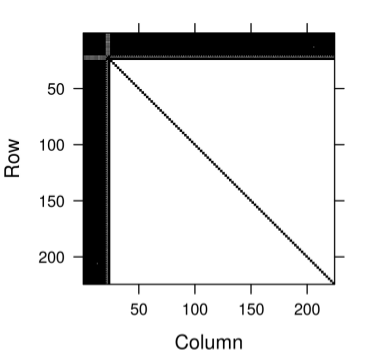
\includegraphics[width=2in]{0_home_rgiordan_Documents_git_repos_Covariances___BPaper_writing_static_images_logit_sparsity.png}\caption{Example sparsity of $\protect\klhess$ for the logit GLMM model (black
indicates non-zero entries)}
\label{fig:LogitGLMMHessianSparsity}
\end{figure}
 

Taking advantage of this sparsity pattern, we used \texttt{autograd}
to calculate the Hessian of the KL divergence one group at a time
and assembled the results in a sparse matrix using the \texttt{scipy.sparse}
Python package. Even so, calculating the entire sparse Hessian took
$\glmmHessianTime$ seconds, and solving the system $\klhess^{-1}\eggrad^{\trans}$
using \texttt{scipy.sparse.linalg.spsolve} took an additional $\glmmInverseTime$
seconds. This means that the evaluation and inversion of $\klhess$
was several times more costly than optimizing the variational objective
itself. (Of course, the whole procedure remains much faster than running
MCMC with Stan.)

We note, however, that instead of the direct approach to calculating
$\klhess^{-1}\eggrad^{\trans}$ one can use the conjugate gradient
algorithm of \texttt{sp.sparse.linalg.cg} \citep[Chapter 5]{nocedalwright:1999:numerical}
together with the fast Hessian-vector products of \texttt{autograd}
to query one column at a time of $\klhess^{-1}\eggrad^{\trans}$.
On a typical column of $\klhess^{-1}\eggrad^{\trans}$ in our experiment,
calculating the conjugate gradient took only $\glmmCGRowTime$ seconds
(corresponding to $\glmmCGRowIters$ Hessian-vector products in the
conjugate gradient algorithm). Thus, for example, one could calculate
the columns of $\klhess^{-1}\eggrad^{\trans}$ corresponding to the
expectations of the global variables $\beta$ in only $\glmmCGRowTime\times K_{x}=\glmmCGBetaTime$
seconds, which is much less time than it would take to compute the
entire $\klhess^{-1}\eggrad^{\trans}$ for both $\beta$ and every
random effect in $u$.

For an additional comparison with MFVB, we also calculated the MAP
estimate:
\begin{align*}
\theta_{map} & :=\argmax_{\theta}\pthetapost\left(\theta\right)=\argmax_{\theta}\log\pthetapost\left(\theta\right).
\end{align*}
We take $\gtheta[\theta_{map}]$ to be the MAP estimate of $\epgtheta$.
The MAP estimator $\theta_{map}$, like the variational approximation
$\qthetapost\left(\theta\right)$, is found by solving an optimization
problem that does not require the normalizing constant of $\pthetapost\left(\theta\right)$.
Indeed, the MAP estimator can be seen as equivalent to a MFVB approximation
in which every parameter has a degenerate distribution that concentrates
at a single point \citep{neal:1998:variationalEM}. Consequently,
the MFVB approximation to posterior means would only be expected to
improve on the MAP estimator in cases when there is both substantial
uncertainty in some parameters and when this uncertainty, through
nonlinear dependence between parameters, affects the values of posterior
means. These circumstances obtain in the logistic GLMM model with
sparse per-advertiser data, since the random effects $u_{t}$ will
be quite uncertain, and the other posterior means depend on them through
the nonlinear logistic function. We calculated the MAP estimator using
the same Python code used for the MFVB estimates.

\subsection{Posterior approximation results\label{subsec:glmm_Means-and-variances}}

In this section, we assess the accuracy of the MFVB and MAP estimators
as approximations to $\epgtheta$ and $\cov_{\pthetapost}\left(\gtheta\right)$,
taking the MCMC estimates as ground truth. Although, as discussed
in \prettyref{subsec:glmm_model}, we are principally interested in
the parameters $\gtheta=\left(\beta^{\trans},u_{1},...,u_{T}\right)^{\trans}$,
we will report the results for all parameters for completeness. For
readability, the tables and graphs show results for a random selection
of the components of the random effects $u$.

\subsubsection{Posterior means}

\begin{table}
\begin{center}% latex table generated in R 3.4.1 by xtable 1.8-2 package
% Thu Sep  7 20:54:26 2017
\begin{tabular}{lrrrrr}
  \hline
Parameter & MCMC & MFVB & MAP & MCMC std. err. & Eff. \# of MCMC draws \\ 
  \hline
$\beta_{1}$ & 1.454 & 1.447 & 1.899 & 0.02067 & 33 \\ 
  $\beta_{2}$ & 0.031 & 0.033 & 0.198 & 0.00025 & 5000 \\ 
  $\beta_{3}$ & 0.110 & 0.110 & 0.103 & 0.00028 & 5000 \\ 
  $\beta_{4}$ & -0.172 & -0.173 & -0.173 & 0.00016 & 5000 \\ 
  $\beta_{5}$ & 0.273 & 0.273 & 0.280 & 0.00042 & 5000 \\ 
  $\mu$ & 2.041 & 2.041 & 3.701 & 0.04208 & 28 \\ 
  $\tau$ & 0.892 & 0.823 & 827.724 & 0.00051 & 1232 \\ 
  $u_{1431}$ & 1.752 & 1.757 & 3.700 & 0.00937 & 5000 \\ 
  $u_{4150}$ & 1.217 & 1.240 & 3.699 & 0.01022 & 5000 \\ 
  $u_{4575}$ & 2.427 & 2.413 & 3.702 & 0.00936 & 5000 \\ 
  $u_{4685}$ & 3.650 & 3.633 & 3.706 & 0.00862 & 5000 \\ 
   \hline
\end{tabular}
\end{center}
\caption{Results for the estimation of the posterior means\label{tab:mean_results}}
\end{table}

\begin{knitrout}
\definecolor{shadecolor}{rgb}{0.969, 0.969, 0.969}\color{fgcolor}\begin{figure}[!h]

{\centering 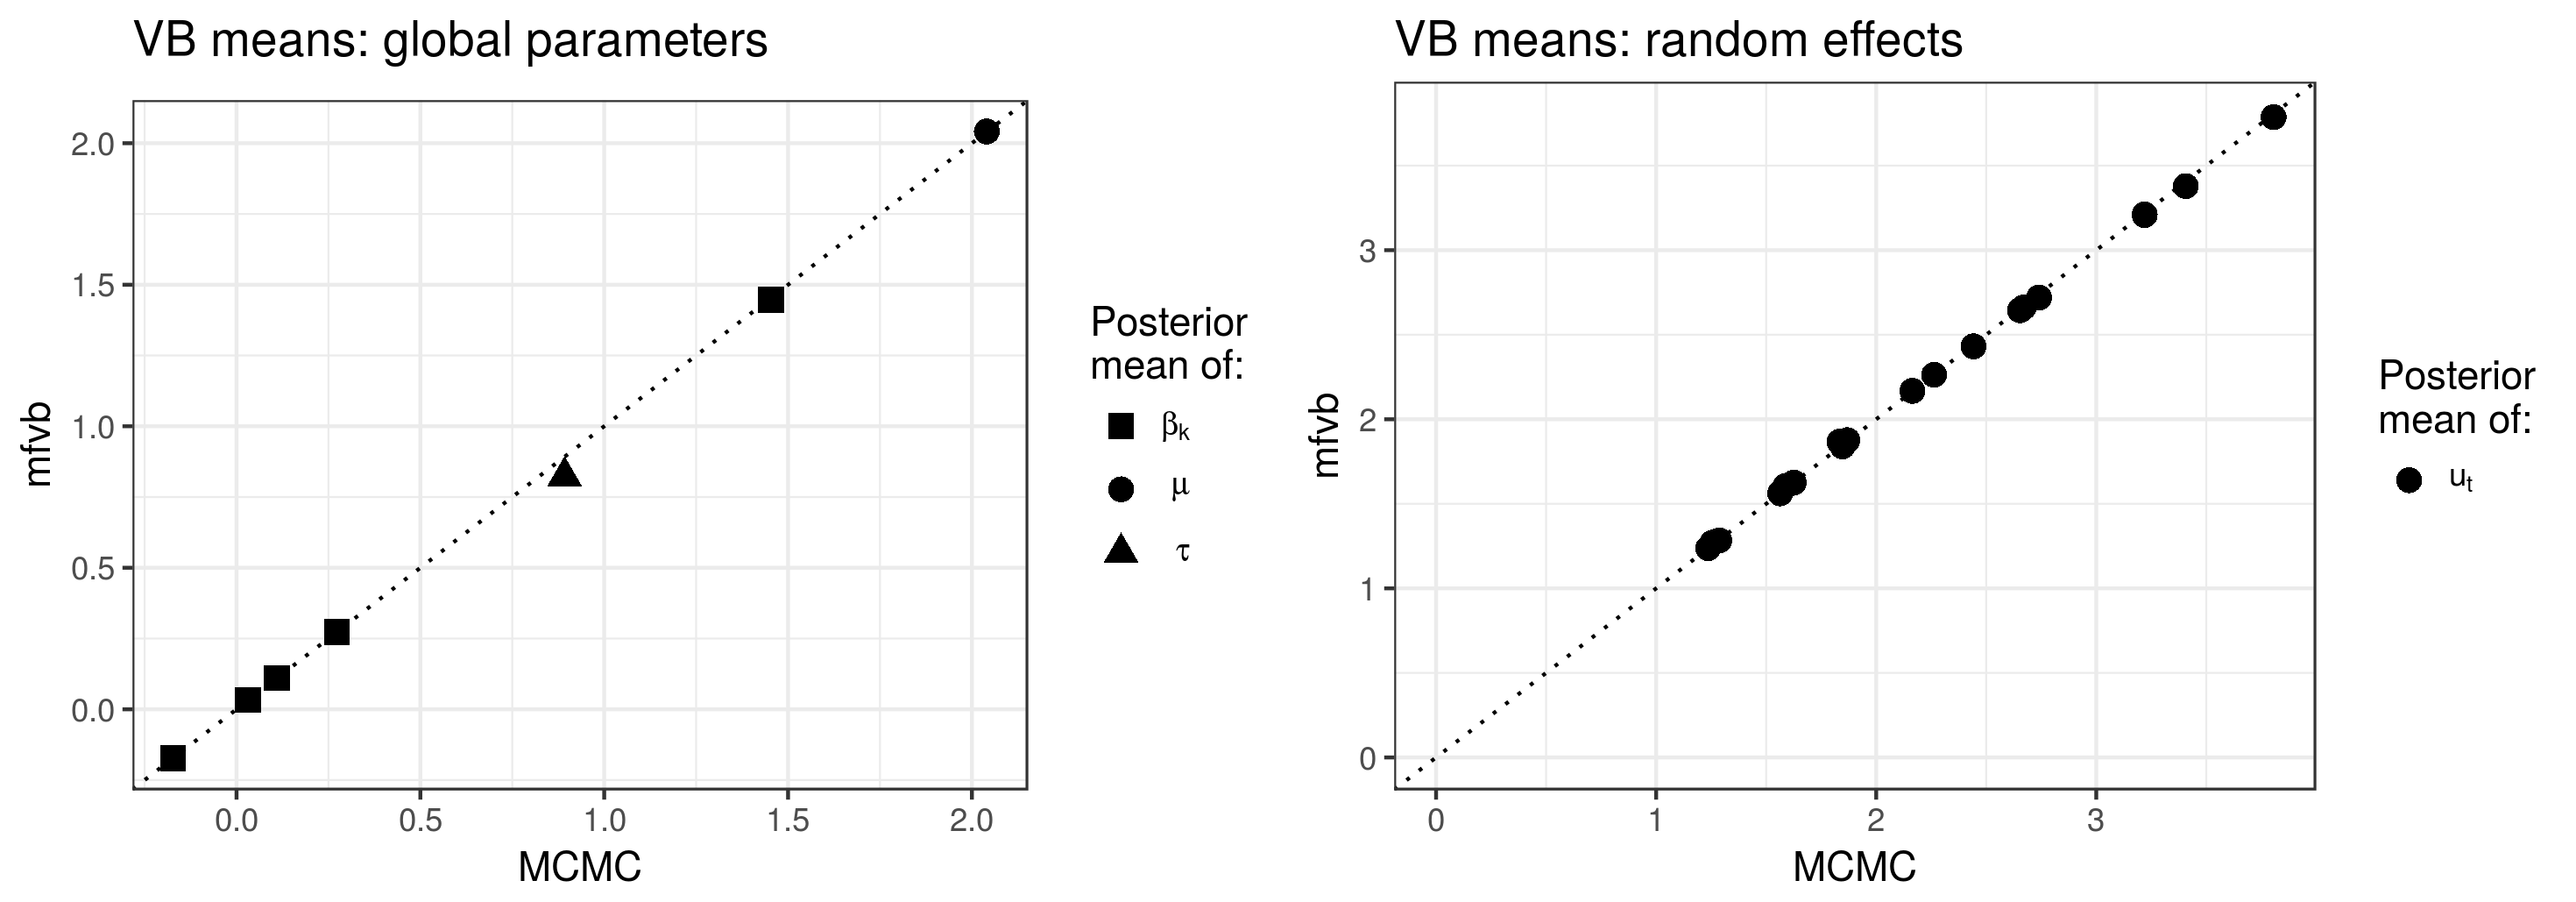
\includegraphics[width=0.98\linewidth,height=0.343\linewidth]{figure/LogitGLMMMCMCComparisonMeans-1} 

}

\caption[Comparison of MCMC and MFVB means]{Comparison of MCMC and MFVB means}\label{fig:LogitGLMMMCMCComparisonMeans}
\end{figure}


\end{knitrout}

\begin{knitrout}
\definecolor{shadecolor}{rgb}{0.969, 0.969, 0.969}\color{fgcolor}\begin{figure}[!h]

{\centering 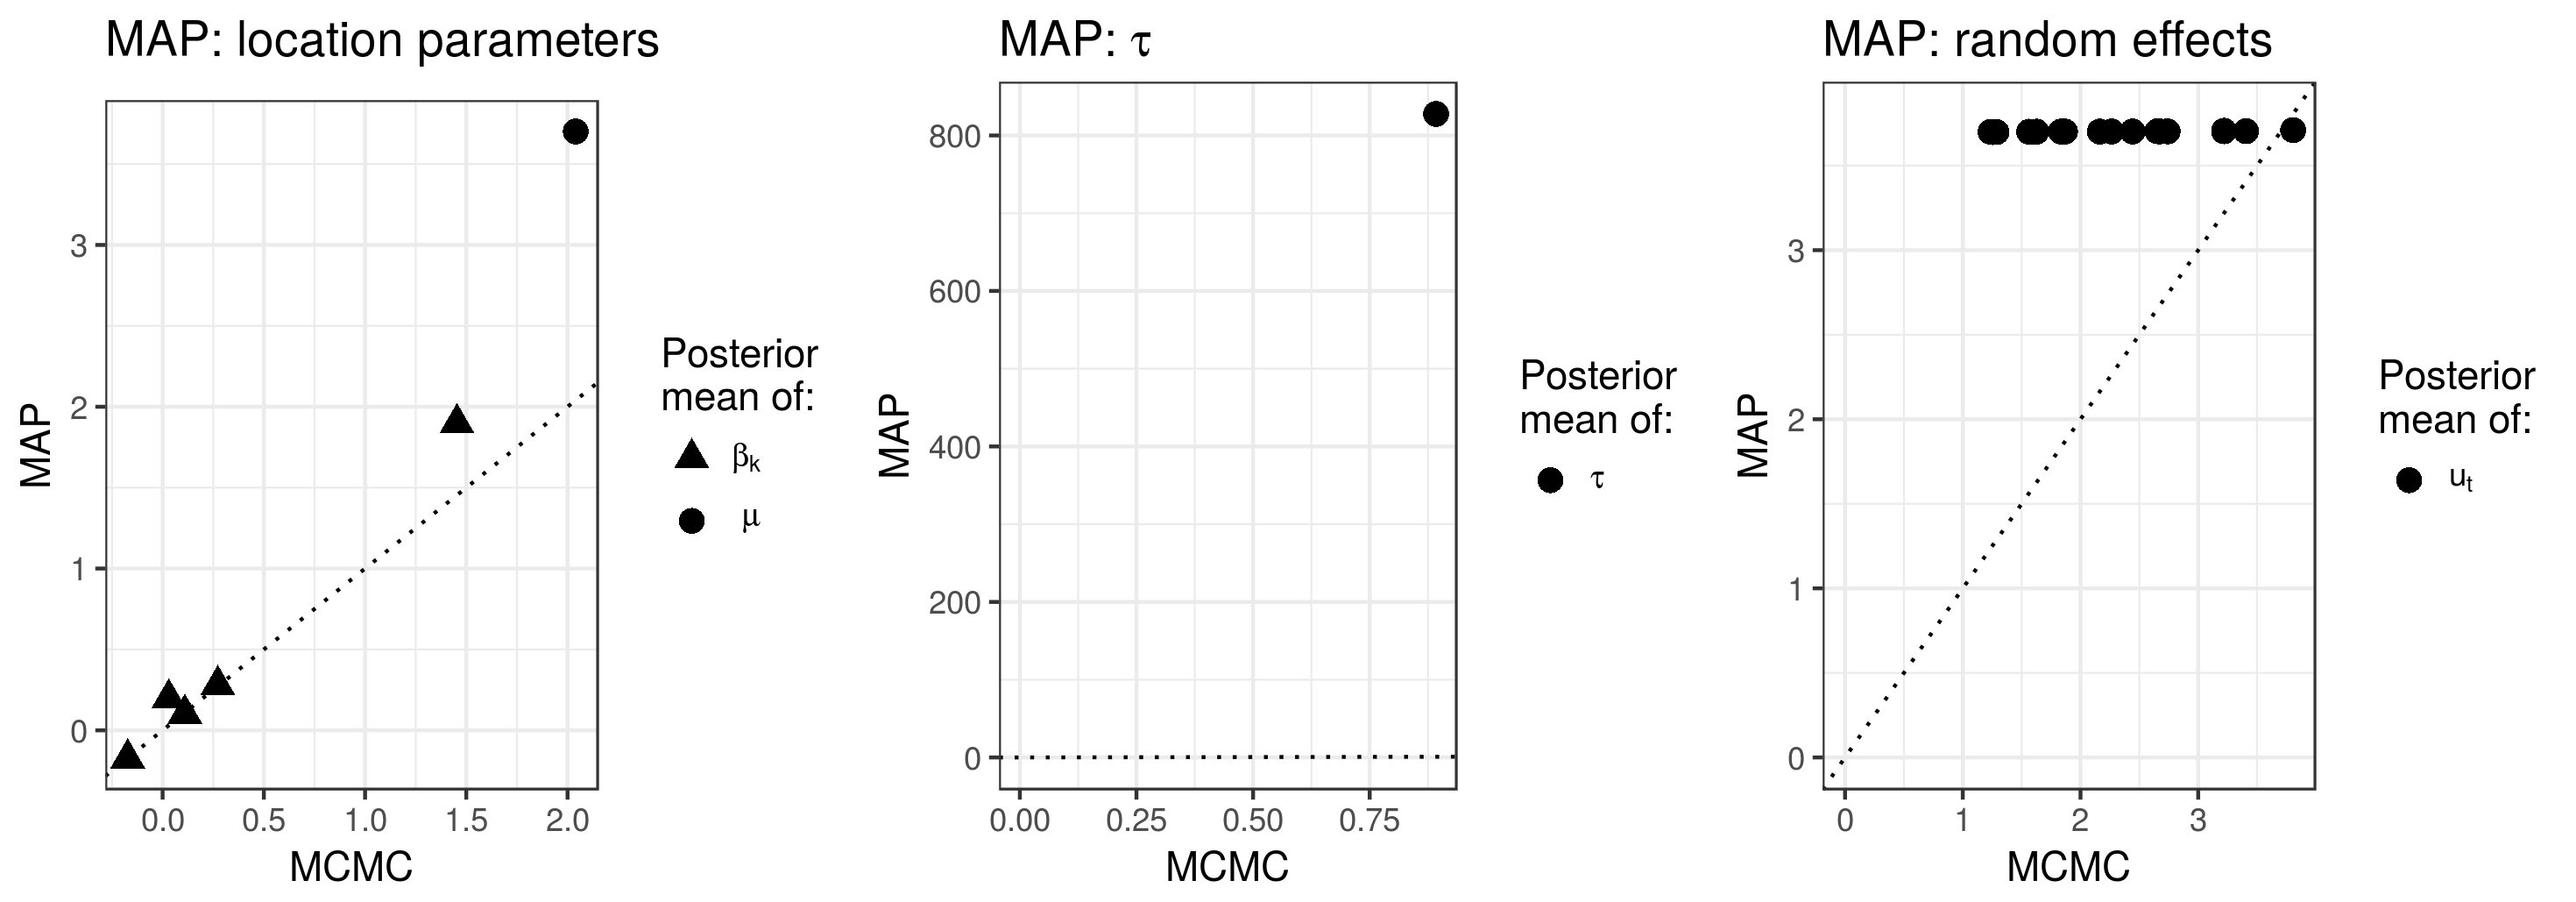
\includegraphics[width=0.98\linewidth,height=0.343\linewidth]{figure/LogitGLMMMapComparisonMeans-1} 

}

\caption[Comparison of MCMC and MAP means]{Comparison of MCMC and MAP means}\label{fig:LogitGLMMMapComparisonMeans}
\end{figure}


\end{knitrout}

We begin by comparing the posterior means in \prettyref{tab:mean_results},
\fig{LogitGLMMMCMCComparisonMeans} and \fig{LogitGLMMMapComparisonMeans}.
We first note that, despite the long running time for MCMC, the $\beta_{1}$
and $\mu$ parameters did not mix well in the MCMC sample, as is reflected
in the MCMC standard error and effective number of draws columns of
\prettyref{tab:mean_results}. The $x_{it}$ data corresponding to
$\beta_{1}$ contained fewer distinct values than the other columns
of $x$, which perhaps led to some co-linearity between $\beta_{1}$
and $\mu$ in the posterior. This could have caused both poor MCMC
mixing and, perhaps, excessive prior sensitivity, as discussed below
in \prettyref{subsec:glmm_sensitivity}. Although we will report the
results for both $\beta_{1}$ and $\mu$ without further comment,
the reader should bear in mind that the MCMC ``ground truth'' for
these two parameters is somewhat suspect.

The results in \prettyref{tab:mean_results} and \fig{LogitGLMMMCMCComparisonMeans}
show that MFVB does an excellent job of approximating the posterior
means in this particular case, even for the random effects $u$ and
the related parameters $\mu$ and $\tau$. In contrast, the MAP estimator
does reasonably well only for certain components of $\beta$ and does
extremely poorly for the random effects parameters. As can be seen
in \fig{LogitGLMMMapComparisonMeans}, the MAP estimate dramatically
overestimates the information $\tau$ of the random effect distribution
(that is, it underestimates the variance). As a consequence, it estimates
all the random effects to have essentially the same value, leading
to mis-estimation of some location parameters, including both $\mu$
and some components of $\beta$. Because the MAP estimator performed
so poorly at estimating the random effect means, we will not consider
it any further.

\subsubsection{Posterior covariances}

\begin{table}
\begin{center}% latex table generated in R 3.4.1 by xtable 1.8-2 package
% Thu Sep  7 20:54:29 2017
\begin{tabular}{lrrr}
  \hline
Parameter & MCMC & LRVB & Uncorrected MFVB \\ 
  \hline
$\beta_{1}$ & 0.118 & 0.103 & 0.005 \\ 
  $\beta_{2}$ & 0.018 & 0.018 & 0.004 \\ 
  $\beta_{3}$ & 0.020 & 0.020 & 0.004 \\ 
  $\beta_{4}$ & 0.012 & 0.012 & 0.004 \\ 
  $\beta_{5}$ & 0.029 & 0.030 & 0.004 \\ 
  $\mu$ & 0.223 & 0.192 & 0.016 \\ 
  $\tau$ & 0.018 & 0.033 & 0.016 \\ 
  $u_{1431}$ & 0.663 & 0.649 & 0.605 \\ 
  $u_{4150}$ & 0.723 & 0.707 & 0.662 \\ 
  $u_{4575}$ & 0.662 & 0.649 & 0.615 \\ 
  $u_{4685}$ & 0.610 & 0.607 & 0.579 \\ 
   \hline
\end{tabular}
\end{center}
\caption{Standard deviation results\label{tab:sd_results}}
\end{table}
\begin{knitrout}
\definecolor{shadecolor}{rgb}{0.969, 0.969, 0.969}\color{fgcolor}\begin{figure}[!h]

{\centering 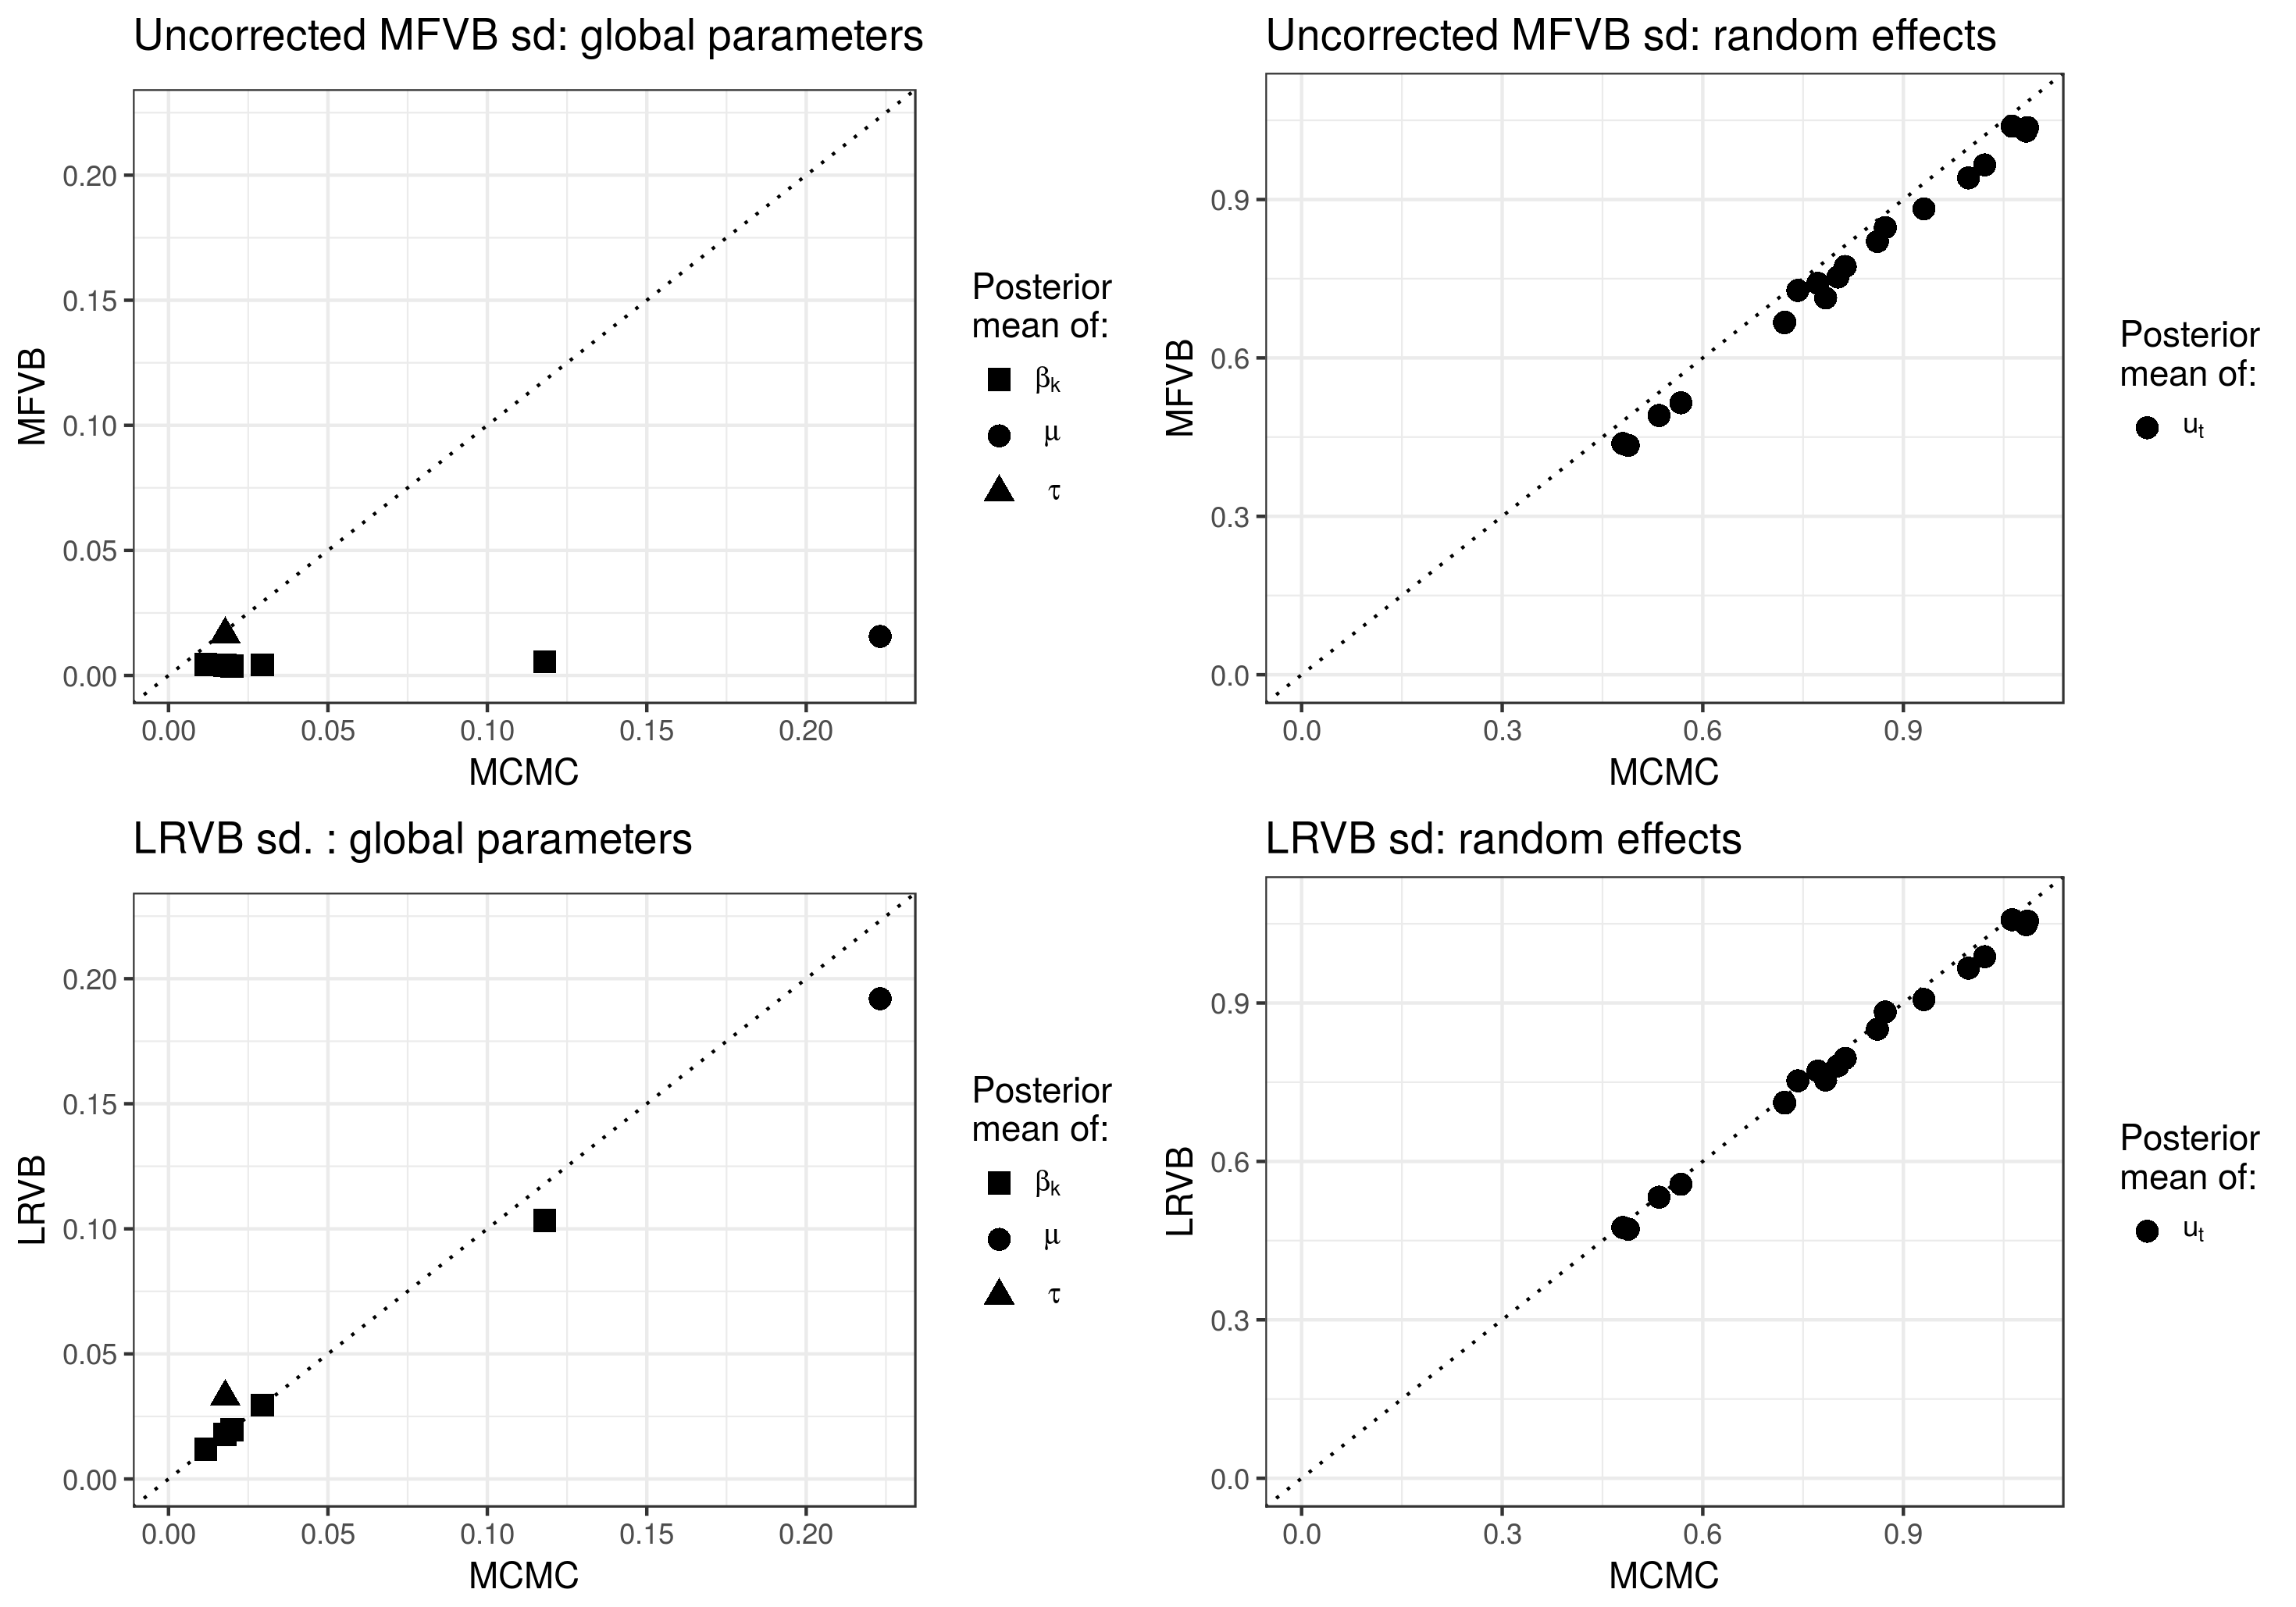
\includegraphics[width=0.98\linewidth,height=0.686\linewidth]{figure/LogitGLMMMCMCComparisonSds-1} 

}

\caption[Comparison of MCMC, MFVB, and LRVB standard deviations]{Comparison of MCMC, MFVB, and LRVB standard deviations}\label{fig:LogitGLMMMCMCComparisonSds}
\end{figure}


\end{knitrout}

\begin{knitrout}
\definecolor{shadecolor}{rgb}{0.969, 0.969, 0.969}\color{fgcolor}\begin{figure}[!h]

{\centering 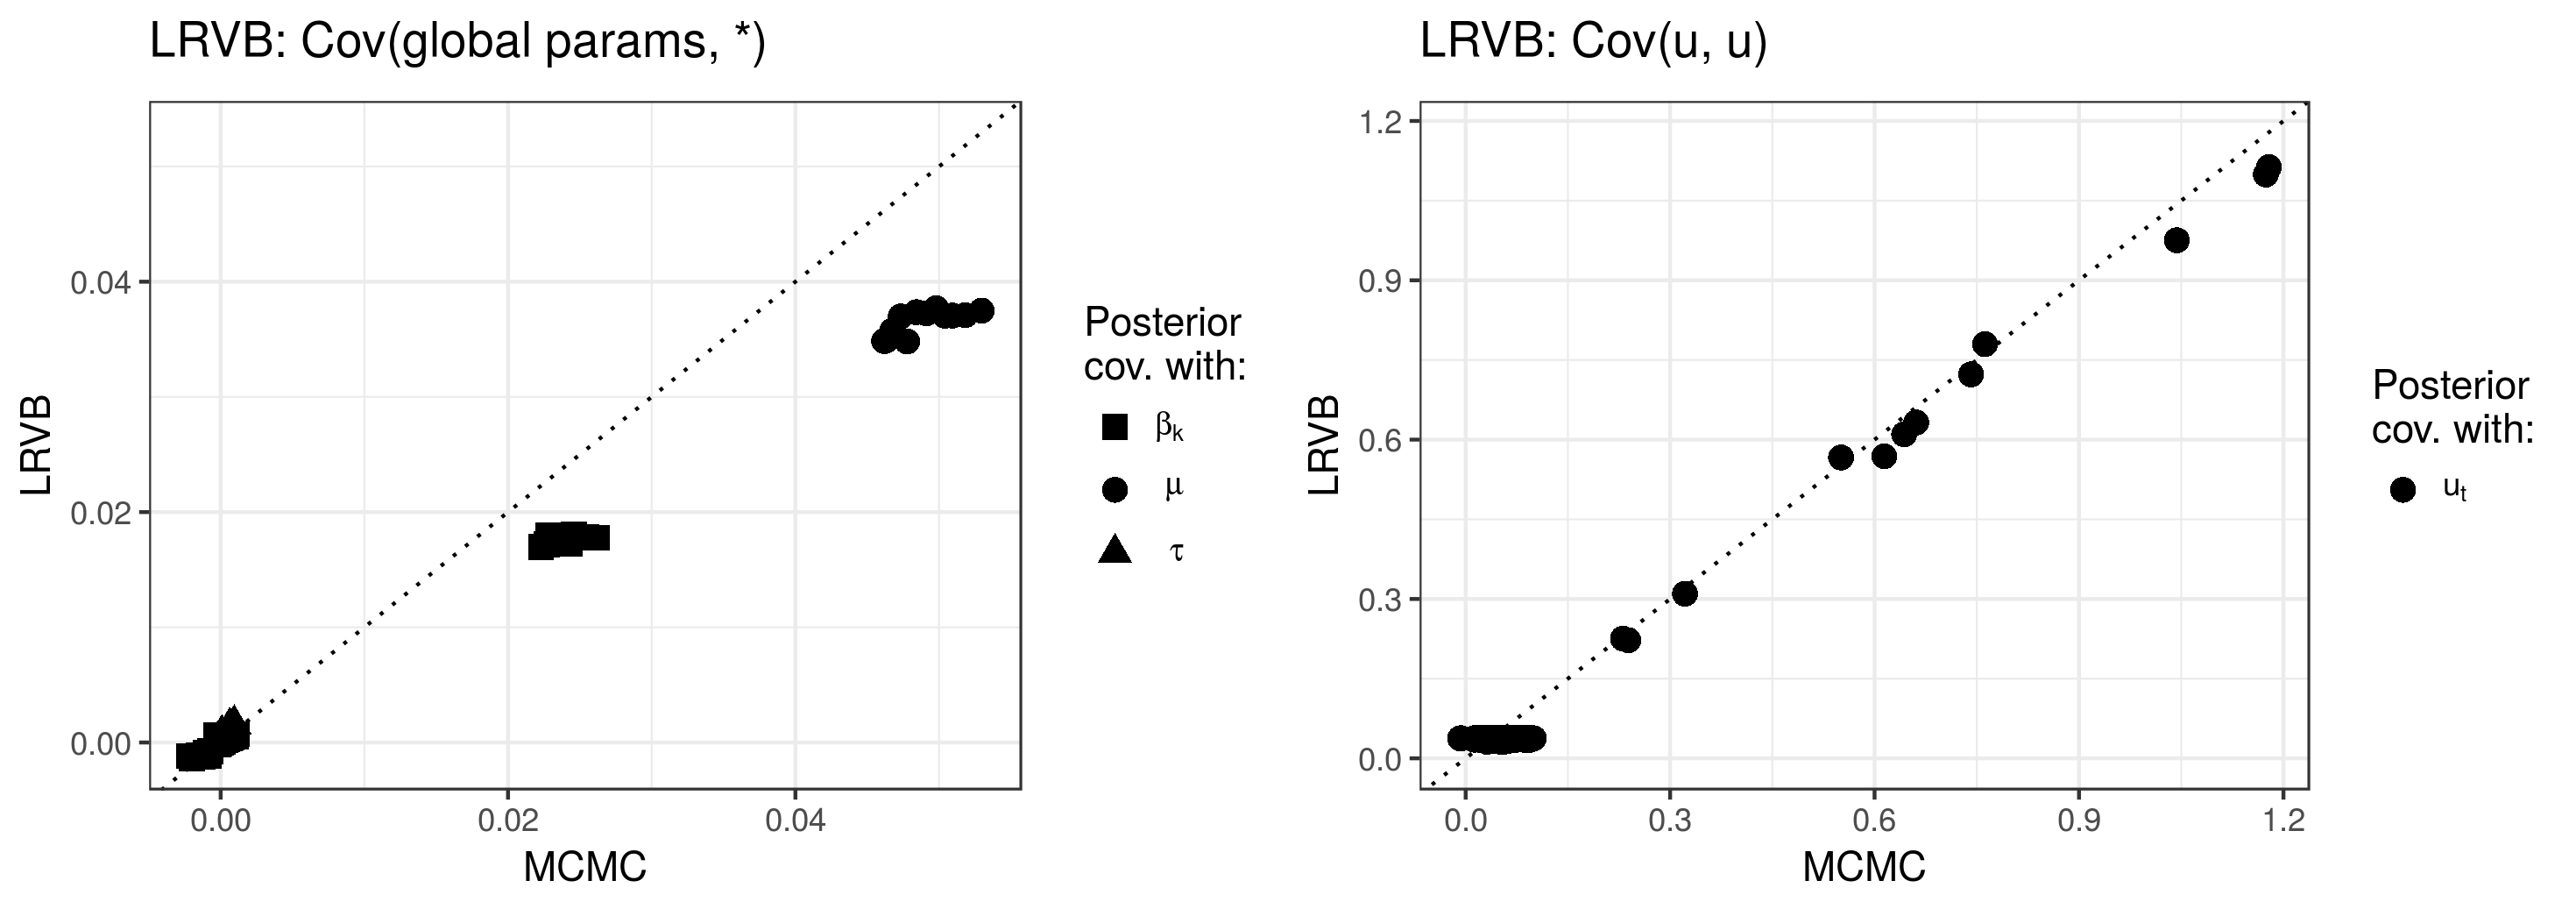
\includegraphics[width=0.98\linewidth,height=0.343\linewidth]{figure/LogitGLMMMCMCComparisonCovariances-1} 

}

\caption[Comparison of MCMC and LRVB off-diagonal covariances]{Comparison of MCMC and LRVB off-diagonal covariances}\label{fig:LogitGLMMMCMCComparisonCovariances}
\end{figure}


\end{knitrout}
We now assess the accuracy of our estimates of $\cov_{\pthetapost}\left(\gtheta\right)$.
The results for the diagonals (i.e., the marginal variances) are shown
in \prettyref{tab:sd_results} and \fig{LogitGLMMMCMCComparisonSds}.
We refer to the diagonal of $\cov_{\qthetapost}\left(\gtheta\right)$
as the ``uncorrected MFVB'' estimate, and the diagonal of the linear
response covariance estimate $\lrvbcov\left(\gtheta\right)$ of \prettyref{def:lrvb_covariance}
as the ``LRVB'' estimate. To make the scale more meaningful, we
report standard deviations rather than variances. The uncorrected
MFVB variance estimates $\var_{\qthetapost}\left(\beta\right)$ are
particularly inaccurate, but the LRVB variances match the true posterior
closely.

In \fig{LogitGLMMMCMCComparisonCovariances}, we compare the off-diagonal
elements of $\lrvbcov\left(\gtheta\right)$ and $\cov_{\pthetapost}\left(\gtheta\right)$.
These covariances are zero, by definition, in the uncorrected MFVB
estimates $\cov_{\qthetapost}\left(\gtheta\right)$. The left panel
of \fig{LogitGLMMMCMCComparisonCovariances} shows the estimated covariances
between the global parameters and all other parameters, including
the random effects, and the right panel shows only the covariances
amongst the random effects. The LRVB covariances are quite accurate,
particularly recalling that the MCMC draws of $\mu$ may be inaccurate
due to poor mixing.

\subsection{Parametric sensitivity results\label{subsec:glmm_sensitivity}}

\begin{table}
\begin{center}% latex table generated in R 3.4.1 by xtable 1.8-2 package
% Thu Sep  7 20:54:31 2017
\begin{tabular}{lrrrrrrr}
  \hline
  & $\beta_{0}$ & $\tau_{\beta}$ & $\gamma_{\beta}$ & $\mu_0$ & $\tau_{\mu}$ & $\alpha_{\tau}$ & $\beta{\tau}$ \\ 
  \hline
$\mu$ & 0.0094 & -0.1333 & -0.0510 & 0.0019 & -0.3920 & 0.0058 & -0.0048 \\ 
  $\tau$ & 0.0009 & -0.0086 & -0.0142 & 0.0003 & -0.0575 & 0.0398 & -0.0328 \\ 
  $\beta_{1}$ & 0.0089 & -0.1464 & -0.0095 & 0.0017 & -0.3503 & 0.0022 & -0.0018 \\ 
  $\beta_{2}$ & 0.0012 & -0.0143 & -0.0113 & 0.0003 & -0.0516 & 0.0062 & -0.0051 \\ 
  $\beta_{3}$ & -0.0035 & 0.0627 & -0.0081 & -0.0006 & 0.1218 & -0.0003 & 0.0002 \\ 
  $\beta_{4}$ & 0.0018 & -0.0037 & -0.0540 & 0.0004 & -0.0835 & 0.0002 & -0.0002 \\ 
  $\beta_{5}$ & 0.0002 & 0.0308 & -0.0695 & 0.0002 & -0.0383 & 0.0011 & -0.0009 \\ 
  $u_{1431}$ & 0.0028 & -0.0397 & -0.0159 & 0.0006 & -0.1169 & 0.0018 & -0.0015 \\ 
  $u_{4150}$ & 0.0026 & -0.0368 & -0.0146 & 0.0005 & -0.1083 & 0.0022 & -0.0018 \\ 
  $u_{4575}$ & 0.0028 & -0.0406 & -0.0138 & 0.0006 & -0.1153 & 0.0011 & -0.0009 \\ 
  $u_{4685}$ & 0.0028 & -0.0409 & -0.0142 & 0.0006 & -0.1163 & 0.0003 & -0.0002 \\ 
   \hline
\end{tabular}
\end{center}
\caption{MFVB normalized prior sensitivity results\label{tab:prior_sens}}
\end{table}

\begin{knitrout}
\definecolor{shadecolor}{rgb}{0.969, 0.969, 0.969}\color{fgcolor}\begin{figure}[!h]

{\centering 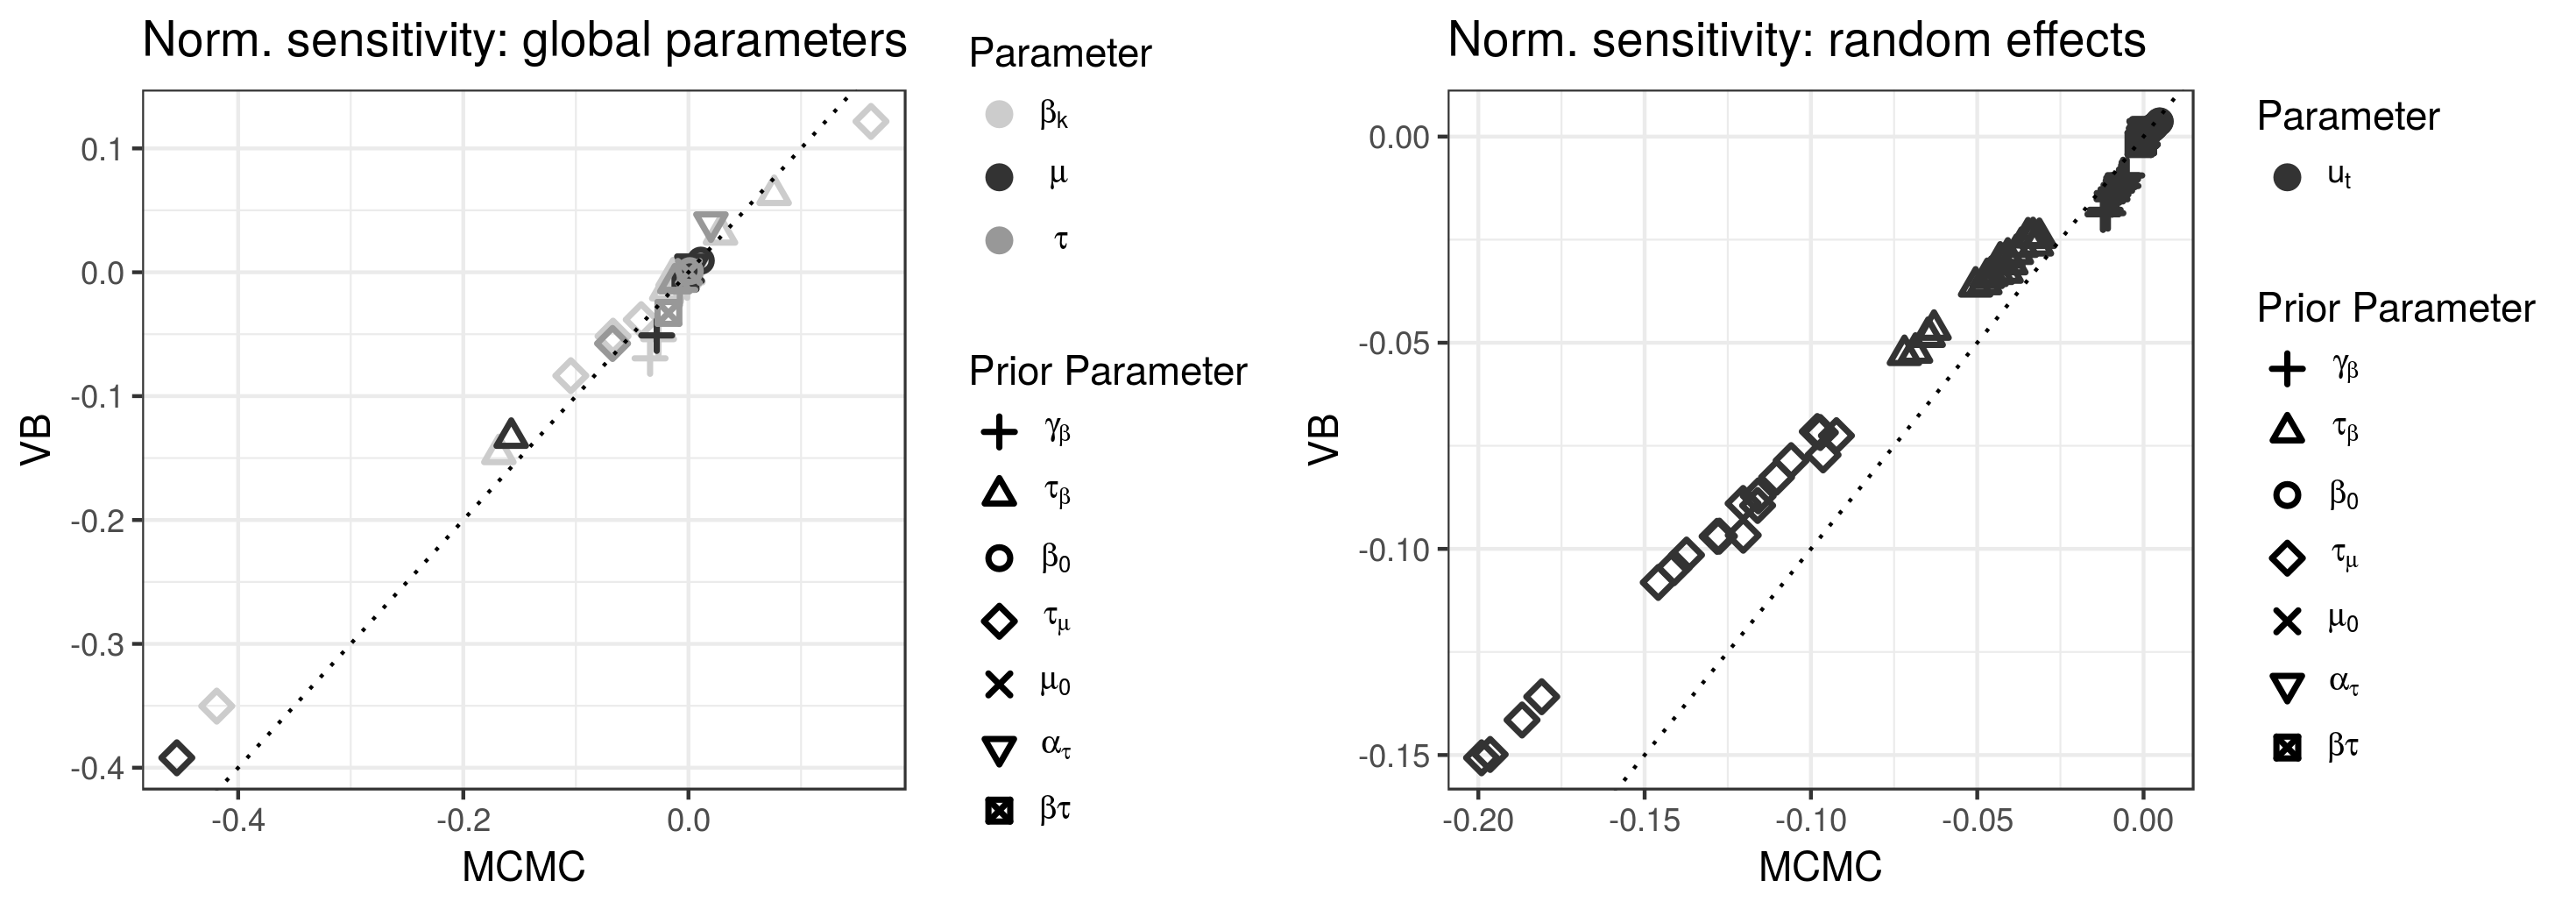
\includegraphics[width=0.98\linewidth,height=0.343\linewidth]{figure/LogitGLMMParametricRobustness-1} 

}

\caption[Comparison of MCMC and MFVB normalized parametric sensitivity results]{Comparison of MCMC and MFVB normalized parametric sensitivity results}\label{fig:LogitGLMMParametricRobustness}
\end{figure}


\end{knitrout}

\begin{knitrout}
\definecolor{shadecolor}{rgb}{0.969, 0.969, 0.969}\color{fgcolor}\begin{figure}[!h]

{\centering 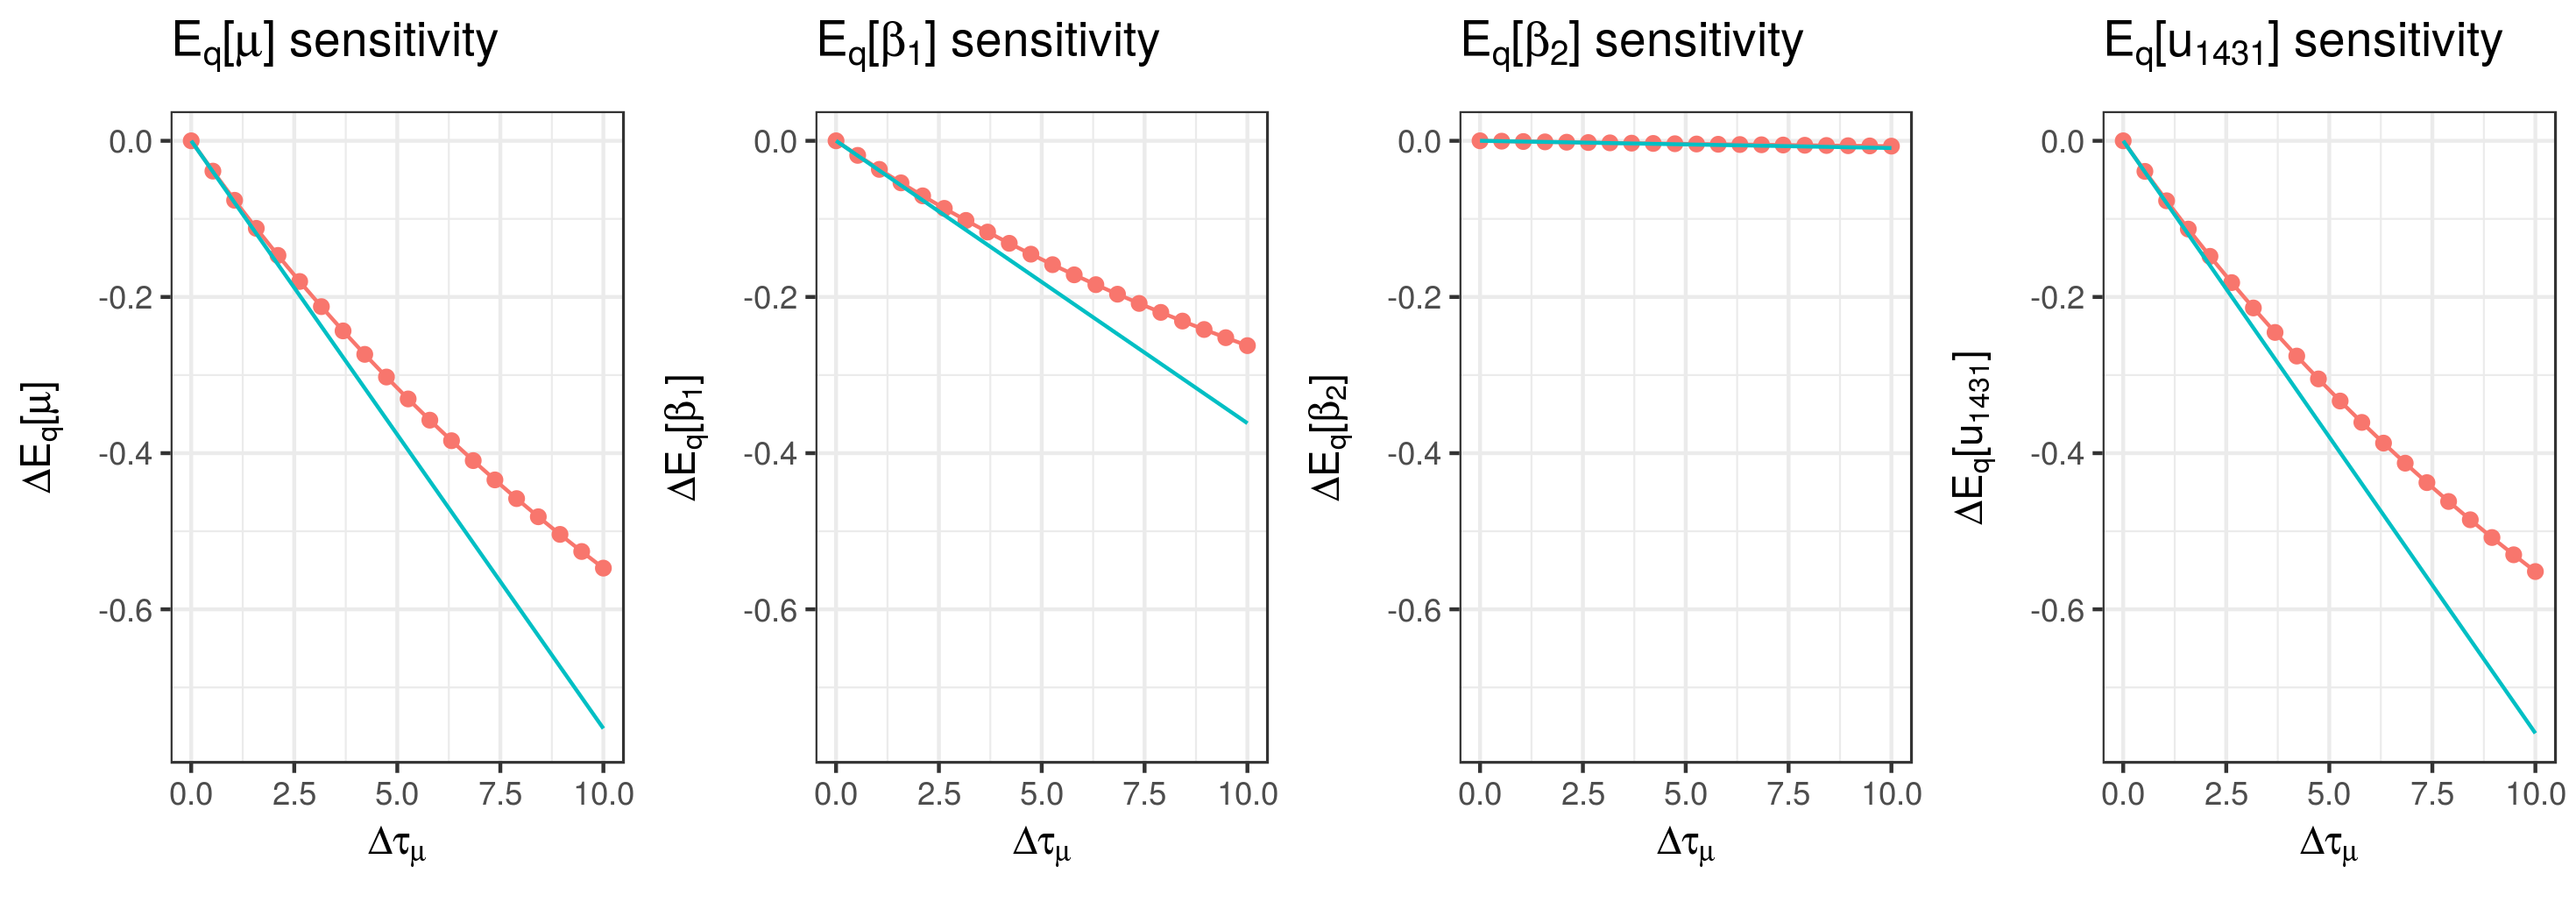
\includegraphics[width=0.98\linewidth,height=0.343\linewidth]{figure/LogitGLMMRefit-1} 

}

\caption[VB sensitivity as measured both by linear approximation and re-fitting]{VB sensitivity as measured both by linear approximation and re-fitting}\label{fig:LogitGLMMRefit}
\end{figure}


\end{knitrout}
Finally, we compare the MFVB prior sensitivity measures of \prettyref{subsec:Parametric-sensitivity}
to the covariance-based MCMC sensitivity measures of \prettyref{subsec:local_sensitivity}.
Since sensitivity is of practical interest only when it is of comparable
order as the posterior uncertainty, we report sensitivities normalized
by the appropriate standard deviation. That is, we report $\psenshat/\sqrt{\textrm{diag}\left(\hat{\cov}_{\pthetapost}\left(\gtheta\right)\right)}$,
and $\qsens/\sqrt{\textrm{diag}\left(\lrvbcov\left(\gtheta\right)\right)}$,
etc., where $\textrm{diag}\left(\cdot\right)$ denotes the diagonal
vector of a matrix, and the division is element-wise. Note that we
use the sensitivity-based variance estimates $\lrvbcov$, not the
uncorrected MFVB estimates $\cov_{\qthetapost}$, to normalize the
variational sensitivities. We refer to a sensitivity divided by a
standard deviation as a ``normalized'' sensitivity. 

The comparison between the MCMC and MFVB sensitivity measures is shown
in \fig{LogitGLMMParametricRobustness}. The MFVB and MCMC sensitivities
correspond very closely, though the MFVB means appear to be slightly
more sensitive to the prior parameters than the MCMC means. This close
correspondence should not be surprising. As shown in \prettyref{subsec:glmm_Means-and-variances},
the MFVB and MCMC posterior means match quite closely. If we assume,
reasonably, that they continue to match in a neighborhood of our original
prior parameters, then \prettyref{assu:vb_accurate} will hold and
we would expect $\psenshat\approx\qsens$.

\prettyref{tab:prior_sens} shows the detailed MFVB normalized sensitivity
results. Each entry is the sensitivity of the VB mean of the row's
parameter to the column's prior parameter. One can see that several
parameters are quite sensitive to the information parameter prior
$\tau_{\mu}.$ In particular, $\mbe_{\pthetapost}\left[\mu\right]$
and $\mbe_{\pthetapost}\left[\beta_{1}\right]$ are expected to change
approximately $-0.39$ and $-0.35$ standard deviations, respectively,
for every unit change in $\tau_{\mu}$. This size of change could
be practically significant (assuming that such a change in $\tau_{\mu}$
is subjectively plausible). To investigate this sensitivity further,
we re-fit the MFVB model at a range of values of the prior parameter
$\tau_{\mu}$, assessing the accuracy of the linear approximation
to the sensitivity. The results are shown in \fig{LogitGLMMRefit}.
Even for very large changes in $\tau_{\mu}$-\textendash -resulting
in changes to $\mbe_{\pthetapost}\left[\mu\right]$ and $\mbe_{\pthetapost}\left[\beta_{1}\right]$
far in excess of two standard deviations-\textendash -the linear approximation
holds up reasonably well. \fig{LogitGLMMRefit} also shows a (randomly
selected) random effect to be quite sensitive, though not to a practically
important degree relative to its posterior standard deviation. The
insensitivity of $\mbe_{\pthetapost}\left[\beta_{2}\right]$ is also
confirmed. Of course, the accuracy of the linear approximation cannot
be guaranteed to hold as well in general as it does in this particular
case, and the quick and reliable evaluation of the linearity assumption
without re-fitting the model remains interesting future work.

Because we started the MFVB optimization close to the new, perturbed
optimum, each new MFVB fit at took only $\glmmVBRefitTime$ seconds
on average. Re-estimating the MCMC posterior so many times would have
been extremely time-consuming. (Note that importance sampling would
be useless for prior parameter changes that moved the posterior so
far from the original draws.) The considerable sensitivity of this
model to a particular prior parameter, which is perhaps surprising
on such a large dataset, illustrates the value of having fast, general
tools for discovering and evaluating prior sensitivity. Our framework
provides just such a set of tools.

\section{Conclusion\label{sec:Conclusion}}

By calculating the sensitivity of VB posterior means to model perturbations,
we are able to provide two important practical tools for VB posterior
approximations: improved variance estimates and measures of prior
robustness. When VB models are implemented in software that supports
automatic differentiation, our methods are fast, scalable, and require
little additional coding beyond the VB objective itself. In our experiments,
we were able to calculate accurate posterior means, covariances, and
prior sensitivity measures orders of magnitude faster than MCMC.

\section{Acknowledgements}

Ryan Giordano's research was supported by the National Energy Research
Scientific Computing Center, a DOE Office of Science User Facility
supported by the Office of Science of the U.S. Department of Energy
under Contract number DE-AC02- 05CH11231. Tamara Broderick's research
was supported in part by a Google Faculty Research Award and the Office
of Naval Research under contract/grant number N00014-17-1-2072. This
work was also supported in part by a MURI award, W911NF-17-1-0304,
from the Army Research Office.

\clearpage{}

\bibliographystyle{plainnat}
\bibliography{variational_robustness}

\clearpage{}


\appendix
\appendixpage

\section{Local sensitivity and covariances\label{app:sens_and_cov}}

In this section we prove \prettyref{thm:sens_cov}. It is a straightforward
consequence of the Lebesgue dominated convergence theorem. Versions
of this theorem have appeared many times before (e.g., \citet{diaconis:1986:consistency,basu:1996:local,gustafson:1996:localposterior,perez:2006:mcmc}
to name a few in the robustness literature).
\begin{assumption}
$\covdens$ is continuously differentiable with respect to $t$, and
there exist $\lambda$-integrable $f_{0}\left(\theta\right)$ and
$f_{1}\left(\theta\right)$ such that $\left|\exp\left(\covdens\right)g\left(\theta\right)\right|<f_{0}\left(\theta\right)$
and $\left|\exp\left(\covdens\right)\right|<f_{1}\left(\theta\right)$.\label{assu:exchange_order}
\end{assumption}

\begin{assumption}
The quantity $\exp\left(\covdens\right)$ can be normalized with respect
to $\lambda$, i.e., $0<\int\exp\left(\covdens\right)\lambda\left(d\theta\right)<\infty$
.\label{assu:bayes_ok}

\end{assumption}

When these assumptions hold for all $t$ in a neighborhood of zero,
we can prove \prettyref{thm:sens_cov}.
\begin{proof}
Under \prettyref{assu:exchange_order}, we can exchange differentiation
and integration in $\int\exp\left(\covdens\right)g\left(\theta\right)\lambda\left(d\theta\right)$
and $\int\exp\left(\covdens\right)\lambda\left(d\theta\right)$ by
\citet[Chapter 5-11, Theorem 18]{fleming:1965:functions}, which ultimately
depends on the Lebesgue dominated convergence theorem. By \prettyref{assu:bayes_ok},
$\mbe_{\covdens}\left[g\left(\theta\right)\right]$ is well-defined
in a neighborhood of $t=0$, and
\begin{align*}
\frac{\partial\exp\left(\covdens\right)}{\partial t} & =\frac{\partial\covdens}{\partial t}\covdens\quad\lambda\textrm{-almost everywhere}.
\end{align*}

Armed with these facts, we can directly compute
\begin{align*}
\left.\frac{\partial\mbe_{\covdens}\left[g\left(\theta\right)\right]}{\partial t^{\trans}}\right|_{t=0} & =\frac{\partial}{\partial t^{\trans}}\left.\frac{\int g\left(\theta\right)\exp\left(\covdens\right)\lambda\left(d\theta\right)}{\int\exp\left(\covdens\right)\lambda\left(d\theta\right)}\right|_{t=0}\\
 & =\left.\frac{\frac{\partial}{\partial t^{\trans}}\int g\left(\theta\right)\exp\left(\covdens\right)\lambda\left(d\theta\right)}{\int\exp\left(\covdens\right)\lambda\left(d\theta\right)}\right|_{t=0}-\mbe_{\covdens}\left[g\left(\theta\right)\right]\left.\frac{\frac{\partial}{\partial t^{\trans}}\int\exp\left(\covdens\right)\lambda\left(d\theta\right)}{\int\exp\left(\covdens\right)\lambda\left(d\theta\right)}\right|_{t=0}\\
 & =\left.\frac{\int g\left(\theta\right)\frac{\partial\covdens}{\partial t^{\trans}}\exp\left(\covdens\right)\lambda\left(d\theta\right)}{\int\exp\left(\covdens\right)\lambda\left(d\theta\right)}\right|_{t=0}-\mbe_{\covdens[][0]}\left[\gtheta\right]\left.\frac{\int\frac{\partial\covdens}{\partial t^{\trans}}\exp\left(\covdens\right)\lambda\left(d\theta\right)}{\int\exp\left(\covdens\right)\lambda\left(d\theta\right)}\right|_{t=0}\\
 & =\cov_{\covdens[][0]}\left(g\left(\theta\right),\left.\frac{\partial\covdens}{\partial t}\right|_{t=0}\right).
\end{align*}
\end{proof}

\section{Comparison with MCMC importance sampling\label{app:mcmc_importance_sampling}}

In this section, we show that using importance sampling with MCMC
samples to calculate the local sensitivity \prettyref{eq:local_robustness}
is precisely equivalent to using the same MCMC samples to estimate
the covariance in \prettyref{eq:covariance_sensitivity_general} directly.
For this section, will suppose that \prettyref{assu:exchange_order}
and \prettyref{assu:bayes_ok} hold. Further suppose, without loss
of generality, we have samples $\theta_{i}$ drawn iid from the normalized
version of $\exp\left(\covdens\right)$:
\begin{align*}
\covdensnorm & :=\frac{\exp\left(\covdens\right)}{\int\exp\left(\covdens[\theta']\right)\lambda\left(d\theta'\right)}\\
\theta_{n} & \iid\covdensnorm[][0],\textrm{ for }n=1,...,N\\
\mbe_{\covdensnorm[][0]}\left[g\left(\theta\right)\right] & \approx\frac{1}{N}\sum_{n=1}^{N}g\left(\theta_{n}\right).
\end{align*}
Define the normalizing constant
\begin{align*}
\tconst & :=\int\exp\left(\covdens[\theta']\right)\lambda\left(d\theta'\right).
\end{align*}
If we could calculate $\tconst$, we could use the following importance
sampling estimate for $\mbe_{\covdensnorm}\left[g\left(\theta\right)\right]$:
\begin{align*}
\mbe_{\covdensnorm}\left[g\left(\theta\right)\right] & \approx\frac{1}{N}\sum_{n=1}^{N}w_{n}g\left(\theta_{n}\right)\\
w_{n} & :=\frac{\covdensnorm[\theta_{n}]}{\covdensnorm[\theta_{n}][0]}\\
 & =\exp\left(\covdens[\theta_{n}]-\covdens[\theta_{n}][0]+\log\tconst[0]-\log\tconst\right).
\end{align*}
Differentiating the weights,

\begin{align*}
\frac{\partial w_{n}}{\partial t} & =w_{n}\left(\frac{\partial\covdens[\theta_{n}]}{\partial t}-\frac{\partial\log\tconst}{\partial t}\right)\\
 & =w_{n}\left(\frac{\partial\covdens[\theta_{n}]}{\partial t}-\frac{1}{\tconst}\int\exp\left(\covdens\right)\frac{\partial\covdens}{\partial t}d\theta\right)\\
 & =w_{n}\left(\frac{\partial\covdens[\theta_{n}]}{\partial t}-\mbe_{\covdensnorm}\left[\frac{\partial\covdens}{\partial t}\right]\right).
\end{align*}
It follows that
\begin{align*}
\left.\frac{\partial}{\partial t}\frac{1}{N}\sum_{n=1}^{N}w_{n}g\left(\theta_{n}\right)\right|_{t=0} & =\frac{1}{N}\sum_{n=1}^{N}\left(\left.\frac{\partial\covdens[\theta_{n}]}{\partial t}\right|_{t=0}-\mbe_{\covdensnorm[][0]}\left[\left.\frac{\partial\covdens}{\partial t}\right|_{t=0}\right]\right)g\left(\theta_{n}\right),
\end{align*}
which is precisely the MCMC sample estimate of the covariance given
by \prettyref{thm:sens_cov}.

\section{Our use of the terms ``sensitivity'' and ``robustness''\label{app:sens_and_robustness}}

In this section we clarify our usage of the terms ``robustness''
and ``sensitivity.'' The quantity $\psens^{\trans}\Delta\alpha$
measures the \emph{sensitivity} of $\epgtheta$ to perturbations in
the direction $\Delta\alpha$. Intuitively, as sensitivity increases,
robustness decreases, and, in this sense, sensitivity and robustness
are opposites of one another. However, we emphasize that sensitivity
is a clearly defined, measurable quantity and that robustness is a
subjective judgment informed by sensitivity, but also by many other
less objective considerations.

Suppose we have calculated the sensitivity to changes in the direction
$\Delta\alpha$ from \prettyref{eq:local_robustness} and found that
it has a particular value. To determine whether our model is robust,
we must additionally decide 
\begin{enumerate}
\item How large of a change in the prior, $||\Delta\alpha||$, is plausible,
and 
\item How large of a change in $\epgtheta$ is important.
\end{enumerate}
The set of plausible prior values necessarily remains a subjective
decision\footnote{This decision can be cast in a formal decision theoretic framework
based on a partial ordering of subjective beliefs. \citep{insua:2012:robustaxioms}}. Whether or not a particular change in $\epgtheta$ is important
depends on the ultimate use of the posterior mean. For example, the
posterior standard deviation can be a guide: if the prior sensitivity
is swamped by the posterior uncertainty then it can be neglected when
reporting our subjective uncertainty about $g\left(\theta\right)$,
and the model is robust. Similarly, even if the prior sensitivity
is much larger than the posterior standard deviation but small enough
that it would not affect any actionable decision made on the basis
of the value of $\epgtheta$, then the model is robust. Intermediate
values remain a matter of judgment. A illustration of the relationship
between sensitivity and robustness is shown in \fig{robustness_vs_sensitivity}.

\begin{figure}
\centering{}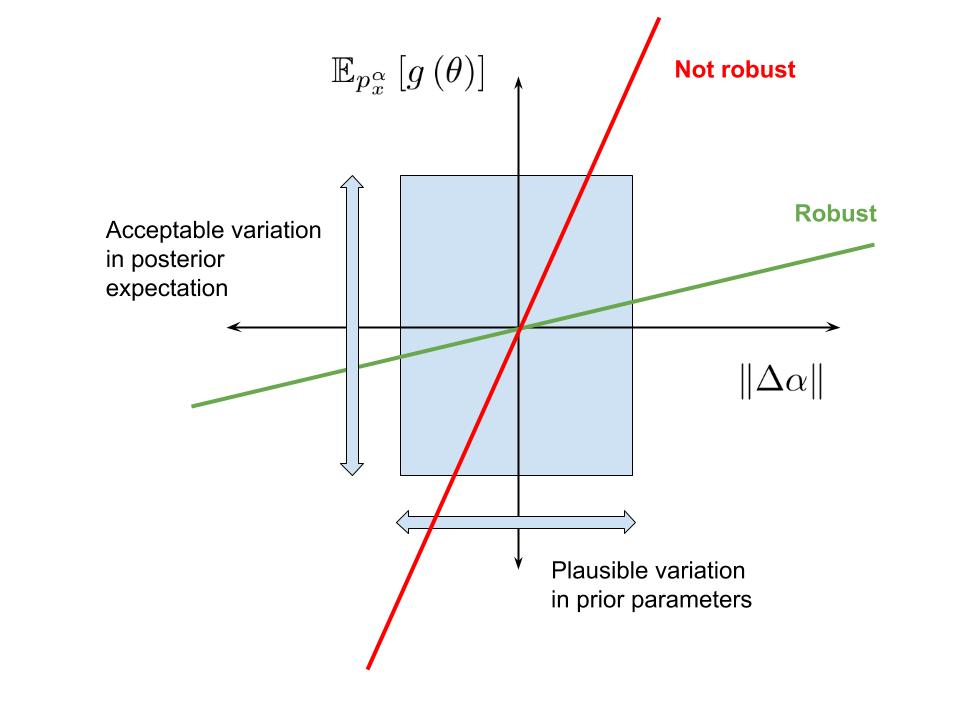
\includegraphics[width=0.5\textwidth]{2_home_rgiordan_Documents_git_repos_Covariances___Paper_writing_static_images_sensitivity_use.jpg}
\caption{The relationship between robustness and sensitivity\label{fig:robustness_vs_sensitivity} }
\end{figure}

Finally, we note that if $\mathcal{A}$ is small enough that $\epgtheta$
is roughly linear in $\alpha$ for $\alpha\in\mathcal{A}$, then calculating
\prettyref{eq:local_robustness} for all $\Delta\alpha\in\mathcal{A}-\alpha$
and finding the worst case can be thought of as a first-order approximation
to a global robustness estimate. Often, this linearity assumption
is not plausible except for very small $\mathcal{A}$, particularly
for function-valued perturbations, as will be seen in \prettyref{sec:experiments}.
This is a weakness inherent to the local robustness approach. Nevertheless,
even when the perturbations are valid only for a small $\mathcal{A}$,
these easily-calculable measures can still provide valuable intuition
about the potential modes of failure for a model.

When the prior has many parameters (i.e., $\alpha$ is high dimensional)
many authors \citep[e.g.][]{basu:1996:local,gustafson:1996:localposterior,roos:2015:sensitivity}
attempt to summarize the high-dimensional vector $\psens$ in a single
easily reported number such as
\begin{align*}
\psens^{sup} & :=\sup_{\alpha:\left\Vert \alpha\right\Vert \le1}\psens.
\end{align*}
Although this summary has obvious merits, in this work we do not attempt
to summarize $\psens$ in this way for several reasons. First of all,
the unit ball $\left\Vert \alpha\right\Vert \le1$ (as in \citet{basu:1996:local})
may not make sense as a subjective description of the range of plausible
variability of $\prior$\textemdash why should the off-diagonal term
of a Wishart prior plausibly vary as widely as the mean of some other
parameter, when the two might not even have the same units? This problem
might be easily remedied by choosing an appropriate scaling of the
parameters and thereby making the unit ball an appropriate range for
the problem at hand, but the right scaling will vary from problem
to problem and necessarily be a somewhat subjective choice, so we
refrain from taking a stand on this decision. 

\section{Variational Bayes sensitivity derivations and assumptions\label{app:lrvb}}

Using the notation from \prettyref{subsec:vb_sensitivity}, we will
make the following assumptions:
\begin{assumption}
The posterior in \prettyref{eq:p_tilting} is well-defined for $t$
in a neighborhood of zero; i.e., there exists some $\delta>0$ such
that \label{assu:tilt_exists}
\begin{eqnarray*}
\int p\left(\theta\vert x\right)p\left(\theta\vert\alpha\right)\exp\left(f\left(\theta,t\right)\right)d\theta & < & \infty,\forall t\in\left\{ t:\left\Vert t\right\Vert _{2}<\delta\right\} .
\end{eqnarray*}
\end{assumption}

\begin{assumption}
There exists a local minimum, $\etaopt$, of $KL\left(q\left(\theta;\eta\right)||\pthetapost\left(\theta\right)\right)$
in \prettyref{eq:kl_divergence}, such that $\etaopt$ is interior
to $\Omega_{\eta}$.\label{assu:opt_interior}
\end{assumption}

\begin{assumption}
The KL divergence, $KL\left(q\left(\theta;\eta\right)||\ptthetapost\left(\theta\right)\right)$
is twice differentiable and strictly convex for $\eta$ in a neighborhood
of the optimal $\etaopt$ and $t$ in a neighborhood of zero. \label{assu:kl_nice}
\end{assumption}

\begin{assumption}
The optimum $\etatopt$ of $KL\left(q\left(\theta;\eta\right)||\ptthetapost\left(\theta\right)\right)$
is a continuously differentiable function of $t$ in a neighborhood
of $\etaopt=\etaopt\left(0\right)$.\label{assu:eta_t_smooth}
\end{assumption}

We now prove \prettyref{thm:lrvb_formula}.
\begin{proof}
Under \prettyref{assu:tilt_exists}, we can define a variational approximation
to the tilted likelihood $\ptthetapost\left(\theta\right)$ that is
a function of $t$: 
\begin{eqnarray*}
\qtthetapost\left(\theta\right) & := & \textrm{argmin}_{q\in\mathcal{Q}}\left\{ KL\left(q\left(\theta;\eta\right)||\ptthetapost\left(\theta\right)\right)\right\} .
\end{eqnarray*}
 For notational convenience, we will define 
\begin{eqnarray*}
KL\left(\eta,t\right) & := & KL\left(q\left(\theta;\eta\right)||\ptthetapost\left(\theta\right)\right).
\end{eqnarray*}

Since by \prettyref{assu:opt_interior} $\etatopt$ is both optimal
and interior for all $t$ in a neighborhood of zero, and by \prettyref{assu:kl_nice}
$KL\left(\eta,t\right)$ is smoothly differentiable in $\eta$, the
first order conditions of the optimization problem \prettyref{eq:kl_divergence}
give:
\begin{eqnarray*}
\left.\frac{\partial KL\left(\eta,t\right)}{\partial\eta}\right|_{\eta=\etatopt} & = & 0.
\end{eqnarray*}
By \prettyref{assu:eta_t_smooth} and \prettyref{assu:kl_nice}, we
can take the total derivative of this vector-valued first order condition
with respect to $t$, getting
\begin{eqnarray*}
\left.\frac{\partial^{2}KL\left(\eta,t\right)}{\partial\eta\partial\eta^{T}}\right|_{\eta=\etatopt}\frac{d\etatopt}{dt^{T}}+\left.\frac{\partial^{2}KL\left(\eta,t\right)}{\partial\eta\partial t^{T}}\right|_{\eta=\etatopt} & = & 0.
\end{eqnarray*}
The strict convexity of $KL\left(\eta,t\right)$ around $\etaopt$
in \prettyref{assu:kl_nice} requires that $\left.\frac{\partial^{2}KL\left(\eta,t\right)}{\partial\eta\partial\eta^{T}}\right|_{\eta=\etatopt}$
be invertible, so by evaluating at $t=0$ and solving we find that
\begin{eqnarray*}
\left.\frac{d\etatopt}{dt^{T}}\right|_{t=0} & = & -\left.\left(\frac{\partial^{2}KL\left(\eta,t\right)}{\partial\eta\partial\eta^{T}}\right)^{-1}\frac{\partial^{2}KL\left(\eta,t\right)}{\partial\eta\partial t^{T}}\right|_{\eta=\etaopt,t=0}.
\end{eqnarray*}
Noting that $\mbe_{\qtthetapost}\left[\gtheta\right]$ is a function
of $\etatopt$, by \prettyref{assu:eta_t_smooth} we have 
\begin{eqnarray*}
\left.\frac{d\mbe_{\qtthetapost}\left[\gtheta\right]}{dt^{T}}\right|_{t=0} & = & \frac{\partial\mbeq\left[g\left(\theta\right)\right]}{\partial\eta}\left.\frac{d\etatopt}{dt^{T}}\right|_{\eta=\etaopt,t=0}.
\end{eqnarray*}
Finally, we observe that 
\begin{eqnarray*}
KL\left(q\left(\theta;\eta\right)||\pthetapost\left(\theta;t\right)\right) & = & \mbeq\left[\log q\left(\theta;\eta\right)-\log p\left(x\vert\theta\right)-\log p\left(\theta\vert\alpha\right)-f\left(\theta,t\right)\right]+\constant\Rightarrow\\
\left.\frac{\partial^{2}KL\left(\eta,t\right)}{\partial\eta\partial t^{T}}\right|_{t=0} & = & -\left.\frac{\partial^{2}\mbeq\left[f\left(\theta,t\right)\right]}{\partial\eta\partial t^{\trans}}\right|_{\eta=\etaopt,t=0}.
\end{eqnarray*}
Here, the term $\constant$ contains quantities that do not depend
on $\eta$. Plugging in gives the desired result.
\end{proof}

\section{Exactness of multivariate normal posterior means\label{app:mvn_exact}}

Here, we show that the MFVB estimate of the posterior means of a multivariate
normal with known covariance is exact and that, as an immediate consequence,
the linear response covariance recovers the exact posterior covariance,
i.e., $\lrvbcov\left(\theta\right)=\cov_{\pthetapost}\left(\theta\right)$.

Suppose we are using MFVB to approximate a non-degenerate multivariate
normal posterior, i.e.,
\begin{align*}
\pthetapost\left(\theta\right) & =\mathcal{N}\left(\theta;\mu,\covmat\right)
\end{align*}
for full-rank $\covmat$. This posterior arises, for instance, given
a multivariate normal likelihood $p\left(x\vert\mu\right)=\prod_{n=1:N}\mathcal{N}\left(x_{n}\vert\theta,\covmat_{x}\right)$
with known covariance $\covmat_{x}$ and a conjugate multivariate
normal prior on the unknown mean parameter $\theta$. Additionally,
even when the likelihood is non-normal or the prior is not conjugate,
the posterior may be closely approximated by a multivariate normal
distribution when a Bayesian central limit theorem can be applied
\citep[Chapter 8]{lecam:2012:asymptotics}. We will consider an MFVB
approximation to $\pthetapost\left(\theta\right)$. Specifically,
let the elements of the vector $\theta\in\mathbb{R}^{K}$ be given
by $\theta_{k}$, for $k=1,...,K$, and take the MFVB normal approximation
with means $m_{k}$ and variances $v_{k}$:
\begin{align*}
\mathcal{Q} & =\left\{ q\left(\theta\right):q\left(\theta\right)=\prod_{k=1}^{K}\mathcal{N}\left(\theta_{k};m_{k},v_{k}\right)\right\} .
\end{align*}
In the notation of \prettyref{eq:q_mean_field_family}, we have $\eta_{k}=\left(m_{k},v_{k}\right)^{\trans}.$
The optimal variational parameters are given by $\eta_{k}^{*}=\left(m_{k}^{*},v_{k}^{*}\right)^{\trans}.$
\begin{lem}
\label{lem:mvn_exact}Let $\pthetapost\left(\theta\right)=\mathcal{N}\left(\theta;\mu,\covmat\right)$
for full-rank $\covmat$; let $\mathcal{Q}=\left\{ q\left(\theta\right):q\left(\theta\right)=\prod_{k=1}^{K}\mathcal{N}\left(\theta_{k};m_{k},v_{k}\right)\right\} $
be the mean field approximating family; and let the optimal parameter
$\etaopt=\left(m^{*},v^{*}\right)$ solve 
\begin{align*}
\etaopt & =\argmin_{\eta:q\left(\theta;\eta\right)\in\mathcal{Q}}KL\left(q\left(\theta;\eta\right)||\pthetapost\left(\theta\right)\right).
\end{align*}
Then $m^{*}=\mu$, i.e., the variational posterior means exactly recover
the exact posterior means and $\etaopt$ is interior.
\end{lem}

\begin{proof}
Let $\textrm{diag}\left(v\right)$ denote the $K\times K$ matrix
with $v$ on the diagonal and zero elsewhere. Using the fact that
the entropy of a univariate normal distribution with variance $v$
is $\frac{1}{2}\log v$ plus a constant, the variational objective
\prettyref{eq:kl_divergence} is given by
\begin{align*}
KL\left(q\left(\theta;\eta\right)||\pthetapost\left(\theta\right)\right) & =\mbe_{q\left(\theta;\eta\right)}\left[-\frac{1}{2}\left(\theta-\mu\right)^{\trans}\covmat^{-1}\left(\theta-\mu\right)\right]+\frac{1}{2}\sum_{k}\log v_{k}+C\\
 & =-\frac{1}{2}\textrm{trace}\left(\covmat^{-1}\mbe_{q\left(\theta;\eta\right)}\left[\theta\theta^{\trans}\right]\right)+\mu^{\trans}\covmat^{-1}\mbe_{q\left(\theta;\eta\right)}\left[\theta\right]+\frac{1}{2}\sum_{k}\log v_{k}+C\\
 & =-\frac{1}{2}\textrm{trace}\left(\covmat^{-1}\left(mm^{\trans}+\textrm{diag}\left(v\right)\right)\right)+\mu^{\trans}\covmat^{-1}m+\frac{1}{2}\sum_{k}\log v_{k}+C\\
 & =-\frac{1}{2}\textrm{trace}\left(\covmat^{-1}\textrm{diag}\left(v\right)\right)-\frac{1}{2}m^{\trans}\covmat^{-1}m+\mu^{\trans}\covmat^{-1}m+\frac{1}{2}\sum_{k}\log v_{k}+C.
\end{align*}
The first order condition for the optimal $m^{*}$ is then
\begin{align*}
\left.\frac{\partial KL\left(q\left(\theta;\eta\right)||\pthetapost\left(\theta\right)\right)}{\partial m}\right|_{m=m^{*},v=v^{*}} & =0\Rightarrow\\
-\covmat^{-1}m^{*}+\covmat^{-1}\mu & =0\Rightarrow\\
m^{*} & =\mu.
\end{align*}
The optimal variances follow similarly: 
\begin{align*}
\left.\frac{\partial KL\left(q\left(\theta;\eta\right)||\pthetapost\left(\theta\right)\right)}{\partial v_{k}}\right|_{m=m^{*},v=v^{*}} & =0\Rightarrow\\
-\frac{1}{2}\left(\covmat^{-1}\right)_{kk}+\frac{1}{2}\frac{1}{v_{k}^{*}} & =0\Rightarrow\\
v_{k}^{*} & =\frac{1}{\left(\covmat^{-1}\right)_{kk}}.
\end{align*}
Clearly, both $m^{*}$ and $v^{*}$ are interior. The same result
can be derived via the variational coordinate ascent updates (\citet[Section 10.1.2]{bishop:2006:pattern}
and \citet[Appendix B]{giordano:2015:lrvb}).
\end{proof}
Next, we show that \prettyref{lem:mvn_exact} holds for all perturbations
in \prettyref{eq:p_tilting} of the form $f\left(\theta,t\right)=t^{\trans}\theta$
and that the assumptions necessary for application of \prettyref{thm:lrvb_formula}
are satisfied.
\begin{lem}
\label{lem:mvn_perturbation_exact}Under the conditions of \prettyref{lem:mvn_exact},
let $\ptthetapost\left(\theta\right)$ be defined from \prettyref{eq:p_tilting}
with $f\left(\theta,t\right)=t^{\trans}\theta$ and let $\qtthetapost\left(\theta\right)$
satisfy \prettyref{eq:perturbed_vb_approximation} with the approximating
family given in \prettyref{lem:mvn_exact}. Then $\mbe_{\qtthetapost}\left[\theta\right]=\mbe_{\ptthetapost}\left[\theta\right]$
and \prettyref{assu:tilt_exists}, \prettyref{assu:opt_interior},
\prettyref{assu:kl_nice}, and \prettyref{assu:eta_t_smooth} are
satisfied for all $t$ in a neighborhood of zero. 
\end{lem}

\begin{proof}
By standard properties of the multivariate normal distribution, $\ptthetapost\left(\theta\right)$
is multivariate normal for any $t$ in a neighborhood of zero when
$f\left(\theta,t\right)=t^{\trans}\theta$. This property holds since
$\theta$ is a sufficient statistic of the multivariate normal distribution,
and the corresponding natural parameter of $\pthetapost\left(\theta\right),$
$\covmat^{-1}\mu$, is interior when $\covmat$ is full-rank. \prettyref{assu:tilt_exists}
follows because the non-degenerate multivariate normal distribution
is normalizable, and, by \prettyref{lem:mvn_exact}, we have that
$\mbe_{\qtthetapost}\left[\theta\right]=\mbe_{\ptthetapost}\left[\theta\right]$
and \prettyref{assu:opt_interior} holds. \prettyref{assu:kl_nice}
can be confirmed by directly inspecting the form of the $\mbeq\left[\log\ptthetapost\left(\theta\right)\right]$
term in the perturbed KL divergence:
\begin{align*}
\mbeq\left[\log\ptthetapost\left(\theta\right)\right] & =-\frac{1}{2}\textrm{trace}\left(\covmat^{-1}\textrm{diag}\left(v\right)\right)-\frac{1}{2}m^{\trans}\covmat^{-1}m+\mu^{\trans}\covmat^{-1}m\\
 & \quad-\frac{1}{2}\sum_{k}\log v_{k}+t^{\trans}m+\constant.
\end{align*}

Here, $\constant$ contains quantities that do not depend on the variational
distribution. Finally, \prettyref{assu:eta_t_smooth} holds because,
as shown in \prettyref{lem:mvn_exact}, $\etaopt$ is a smooth function
of the natural exponential family parameters of $\ptthetapost\left(\theta\right)$,
which are in turn smooth functions of $t$.
\end{proof}
It now follows that the linear response variational covariance exactly
reproduces the exact posterior covariance.
\begin{thm}
\label{thm:mvn_cov_exact}Under the conditions of \prettyref{lem:mvn_exact},
$\lrvbcov\left(\theta\right)=\cov_{\pthetapost}\left(\theta\right)$.
\end{thm}

\begin{proof}
From \prettyref{lem:mvn_perturbation_exact} we have that, for all
$t$ in a neighborhood of zero, $\mbe_{\qtthetapost}\left[\theta\right]=\mbe_{\ptthetapost}\left[\theta\right]$.
It follows that
\begin{align*}
\left.\frac{d\mbe_{\qtthetapost}\left[\theta\right]}{dt}\right|_{t=0} & =\left.\frac{d\mbe_{\ptthetapost}\left[\theta\right]}{dt}\right|_{t=0}.
\end{align*}

Since, as argued in \prettyref{lem:mvn_perturbation_exact}, $\ptthetapost\left(\theta\right)$
is multivariate normal for $t$ in a neighborhood of zero, \prettyref{assu:exchange_order}
and \prettyref{assu:bayes_ok} are satisfied, so we can apply \prettyref{thm:sens_cov}
to get
\begin{align*}
\left.\frac{d\mbe_{\ptthetapost}\left[\theta\right]}{dt}\right|_{t=0} & =\cov_{\pthetapost}\left(\theta\right).
\end{align*}

Finally, since by \prettyref{lem:mvn_perturbation_exact} the conditions
for application of \prettyref{thm:lrvb_formula} are satisfied with
$g\left(\theta\right)=\theta$, we have
\begin{align*}
\left.\frac{d\mbe_{\qtthetapost}\left[\theta\right]}{dt}\right|_{t=0} & =\lrvbcov\left(\theta\right).
\end{align*}

It follows directly that $\lrvbcov\left(\theta\right)=\cov_{\pthetapost}\left(\theta\right)$
.
\end{proof}

\section{LKJ Priors for Covariance Matrices in Mean Field Variational Inference\label{app:lkj}}

\global\long\def\lkjdiagmat{\mathbf{S}}

\global\long\def\lkjcorrmat{\mathbf{R}}

\global\long\def\lkjlocmat{\mathbf{V}}

In this section we briefly derive closed-form expressions for using
an LKJ prior with a Wishart variational approximation.
\begin{prop}
Let $\covmat$ be a $K\times K$ positive definite covariance matrix.
Define the $K\times K$ matrix $\lkjdiagmat$ such that
\begin{align*}
\lkjdiagmat_{ij} & =\begin{cases}
\sqrt{\covmat_{ij}} & \textrm{if }i=j\\
0 & \textrm{otherwise}.
\end{cases}
\end{align*}
Define the correlation matrix $R$ as
\begin{align*}
\lkjcorrmat & =\lkjdiagmat^{-1}\covmat\lkjdiagmat^{-1}.
\end{align*}
Define the LKJ prior on $\lkjcorrmat$ with concentration parameter
$\xi$ \citep{lewandowski:2009:lkj}:
\begin{align*}
p\left(\lkjcorrmat\vert\xi\right) & \propto\left|\lkjcorrmat\right|^{\xi-1}.
\end{align*}
Let $q\left(\covmat\vert\lkjlocmat^{-1},\nu\right)$ be an inverse
Wishart distribution with matrix parameter $\lkjlocmat^{-1}$ and
degrees of freedom $\nu$. Then
\begin{align*}
\mathbb{E}_{q}\left[\log\left|\lkjcorrmat\right|\right] & =\log\left|\lkjlocmat^{-1}\right|-\psi_{K}\left(\frac{\nu}{2}\right)-\sum_{k=1}^{K}\log\left(\left(\lkjlocmat^{-1}\right)_{kk}\right)-K\psi\left(\frac{\nu-K+1}{2}\right)+\constant\\
\mbe_{q}\left[\log p\left(\lkjcorrmat\vert\xi\right)\right] & =\left(\xi-1\right)\mathbb{E}_{q}\left[\log\left|\lkjcorrmat\right|\right],
\end{align*}
where $\constant$ does not depend on $\lkjlocmat$ or $\nu$. Here,
$\psi_{K}$ is the multivariate digamma function.
\end{prop}

\begin{proof}
First note that
\begin{align*}
\log\left|\covmat\right| & =2\log\left|\lkjdiagmat\right|+\log\left|\lkjcorrmat\right|=\sum_{k=1}^{K}\log\lkjdiagmat_{k}^{2}+\log\left|\lkjcorrmat\right|=\sum_{k=1}^{K}\log\covmat_{kk}+\log\left|\lkjcorrmat\right|\Rightarrow\\
\log\left|\lkjcorrmat\right| & =\log\left|\covmat\right|-\sum_{k=1}^{K}\log\covmat_{kk}.
\end{align*}
By properties of the inverse Wishart distribution,
\begin{align*}
E_{q}\left[\log\left|\covmat\right|\right] & =\log\left|\lkjlocmat^{-1}\right|-\psi_{K}\left(\frac{\nu}{2}\right)-K\log2,
\end{align*}
where $\psi_{p}$ is the multivariate digamma function. By the marginalization
property of the inverse Wishart distribution,
\begin{align*}
\covmat_{kk} & \sim\textrm{InverseWishart}\left(\left(\lkjlocmat^{-1}\right)_{kk},\nu-K+1\right)\Rightarrow\\
E_{q}\left[\log\covmat_{kk}\right] & =\log\left(\left(\lkjlocmat^{-1}\right)_{kk}\right)-\psi\left(\frac{\nu-K+1}{2}\right)-\log2.
\end{align*}
Plugging in gives the desired result.
\end{proof}

\section{Logistic GLMM Model Details\label{app:glmm_details}}

In this section we include extra details about the model and analysis
of \prettyref{sec:experiments}. We will continue to use the notation
defined therein. Denoting by $\constant$ constants that do not depend
on the prior parameters, parameters, or data, the log likelihood is

\begin{eqnarray*}
\log p\left(y_{it}\vert u_{t},\beta\right) & = & y_{it}\log\left(\frac{p_{it}}{1-p_{it}}\right)+\log\left(1-p_{it}\right)\\
 & = & y_{it}\rho+\log\left(1-p_{it}\right)+\constant\\
\log p\left(u\vert\mu,\tau\right) & = & -\frac{1}{2}\tau\sum_{t=1}^{T}\left(u_{t}-\mu\right)^{2}-\frac{1}{2}T\log\tau\\
 & = & -\frac{1}{2}\tau\sum_{t=1}^{T}\left(u_{t}^{2}-\mu u_{t}+\mu^{2}\right)-\frac{1}{2}T\log\tau+\constant\\
\log p\left(\mu,\tau,\beta\right) & = & -\frac{1}{2}\sigma_{\mu}^{-2}\left(\mu^{2}+2\mu\mu_{0}\right)+\\
 &  & \left(1-\alpha_{\tau}\right)\tau+\beta_{\tau}\log\tau+\\
 &  & -\frac{1}{2}\left(\textrm{trace}\left(\covmat_{\beta}^{-1}\beta\beta^{T}\right)+2\textrm{trace}\left(\covmat_{\beta}^{-1}\beta_{0}\beta^{T}\right)\right).
\end{eqnarray*}

The prior parameters were taken to be
\begin{align*}
\mu_{0} & =\glmmMuLoc\\
\sigma_{\mu}^{-2} & =\glmmMuInfo\\
\beta_{0} & =\glmmBetaLoc\\
\sigma_{\beta}^{-2} & =\glmmBetaInfoDiag\\
\alpha_{\tau} & =\glmmTauAlpha\\
\beta_{\tau} & =\glmmTauBeta.
\end{align*}

Under the variational approximation, $\rho_{it}$ is normally distributed
given $x_{it}$, with 
\begin{eqnarray*}
\rho_{it} & = & x_{it}^{T}\beta+u_{t}\\
\mbe_{q}\left[\rho_{it}\right] & = & x_{it}^{T}\mbe_{q}\left[\beta\right]+\mbe_{q}\left[u_{t}\right]\\
\textrm{Var}_{q}\left(\rho_{it}\right) & = & \mbe_{q}\left[\beta^{T}x_{it}x_{it}^{T}\beta\right]-\mbe_{q}\left[\beta\right]^{T}x_{it}x_{it}^{T}\mbe_{q}\left[\beta\right]+\textrm{Var}_{q}\left(u_{t}\right)\\
 & = & \mbe_{q}\left[\textrm{tr}\left(\beta^{T}x_{it}x_{it}^{T}\beta\right)\right]-\textrm{tr}\left(\mbe_{q}\left[\beta\right]^{T}x_{it}x_{it}^{T}\mbe_{q}\left[\beta\right]\right)+\textrm{Var}_{q}\left(u_{t}\right)\\
 & = & \textrm{tr}\left(x_{it}x_{it}^{T}\left(\mbe_{q}\left[\beta\beta^{T}\right]-\mbe_{q}\left[\beta\right]\mbe_{q}\left[\beta\right]^{T}\right)\right)+\textrm{Var}_{q}\left(u_{t}\right).
\end{eqnarray*}

We can thus use $n_{MC}=\glmmNumGHPoints$ points of Gauss-Hermite
quadrature to numerically estimate $\mbe_{q}\left[\log\left(1-\frac{e^{\rho}}{1+e^{\rho}}\right)\right]$:
\begin{align*}
\rho_{it,s} & :=\sqrt{\textrm{Var}_{q}\left(\rho_{it}\right)}z_{s}+\mbe_{q}\left[\rho_{it}\right]\\
\mbe_{q}\left[\log\left(1-\frac{e^{\rho_{it}}}{1+e^{\rho_{it}}}\right)\right] & \approx\frac{1}{n_{MC}}\sum_{s=1}^{n_{MC}}\log\left(1-\frac{e^{\rho_{it,s}}}{1+e^{\rho_{it,s}}}\right)
\end{align*}
We found that increasing the number of points used for the quadrature
did not measurably change any of the results. The integration points
and weights were calculated using the \texttt{\textit{numpy.polynomial.hermite}}
module in python \citep{scipy}.
\end{document}
